% !Mode:: "TeX:UTF-8"
\documentclass[bachelor,openany,oneside,color]{style/buaathesis}
% 参考文献
\usepackage{style/gbt7714}
\usepackage{algorithm} 
\usepackage{algpseudocode} 
% 参考文献输出方式,numerical为按照出现顺序,authoryear为按照作者姓名和年份
\citestyle{numerical}
% \citestyle{authoryear}
% 取消链接高亮
\hypersetup{hidelinks}
\newcommand{\us}{\_}

% \begin{itemize}
%     \item We propose a hands-free object manipulation pipeline based on eye-dominated object manipulation methods in virtual reality;
%     \item We design a new 3D UI of the four-leaf Clover menu for switching between the manipulation mode with eye gaze;
%     \item we introduce a head-gaze based translating, gaze-based rotating and re-scaling method;
%     \item we design a user study to evaluate the efficiency and accuracy of our method. 
% \end{itemize}

% \subsection{Manipulation Pipeline}

% 1. object selection [XXX]
%     -head pointing [XXX]
%     -confirmation [XXX]
    
% 2. generate a Four-leaf Clover menu around the object and switch the manipulation mode by using gaze the details in \autoref{sec:Clover}. The user can cancel the selection and back to 1.

% 3. with a selected mode, the user starts a corresponding  manipulation.
%    - translating
%    - rotation
%    - scaling
   
%  the details in \autoref{sec:Manipulation}.  
 
% 4. confirm the manipulation, and go to 2.


% \subsection{Four-leaf Clover menu}\label{sec:Clover}

% - image, description of Clover menu
%     - orientation, depth, arragement
%     - size
%     - order 

% - rationale for 3D UI 
%    - easy for mode switch
%    - easy for gaze control
%    -four options: translating, rotation, scaling, and cancel

% - selection interaction, mode switching detection, switching feed-back: highlights and audio 

% - linear filtering


% \subsection{Manipulation method}\label{sec:Manipulation}

%  -translating  head-eye
    
%  -rotation
%  -scaling

\begin{document}

% 用户信息
% !Mode:: "TeX:UTF-8"

% 学院中英文名,中文不需要“学院”二字
% 院系英文名可从以下导航页面进入各个学院的主页查看
% http://www.buaa.edu.cn/xyykc/index.htm
\school
{计算机}{School of Computer Science and Engineering}

% 专业中英文名
\major
{计算机科学与技术}{Computer Science and Technology}

% 论文中英文标题
\thesistitle
{混合现实头眼协同对象操纵方法设计与实现}
{}
{Design and Implementation of a Head-eye Collaborative Object Manipulation Method in Mixed Reality}
{}

% 作者中英文名
\thesisauthor
{刘兆薰}{Zhaoxun Liu}

% 导师中英文名
\teacher
{王莉莉}{Lili Wang}
% 副导师中英文名
% 注:慎用‘副导师’,见北航研究生毕业论文规范
%\subteacher{副导师}{subteacher}

% 中图分类号,可在 http://www.ztflh.com/ 查询
\category{TP312}

% 本科生为毕设开始时间;研究生为学习开始时间
\thesisbegin{2011}{09}{01}

% 本科生为毕设结束时间;研究生为学习结束时间
\thesisend{2012}{07}{01}

% 毕设答辩时间
\defense{2012}{06}{01}

% 中文摘要关键字
\ckeyword{北航开源俱乐部,\LaTeX{},论文}

% 英文摘要关键字
\ekeyword{BHOSC, \LaTeX{}, Thesis}

% !Mode:: "TeX:UTF-8"

% 班级
\class{190614}

% 学号
\studentID{19373345}

% 单位代码
\unicode{10006}

% 论文时间,用于首页
\thesisdate{2023}{05}


% 任务书信息
% !Mode:: "TeX:UTF-8"
% 任务书中的信息
%% 原始资料及设计要求
\assignReq
{针对虚拟现实设计并实现一套基于头眼协同的高效易用的对象操纵方法}
{使用C\# 在Unity3D引擎中进行交互系统逻辑与代码开发}
{使用SteamVR进行相关虚拟现实场景开发}
{使用VIVE Focus 3眼动仪获取、分析眼动数据}
{}
%% 工作内容
\assignWork
{头眼协同的场景与目标浏览}
{头眼协同的目标选择}
{头眼协同的对象操纵}
{两个先导实验}
{两个用户实验}
{对比目前国际一流方法并分析结果}
%% 参考文献
\assignRef
{M. Daniel, C. Ariel, G. Andrea, et al. A survey on 3d virtual object manipulation: }
{From the desktop to immersive virtual environments: Survey on 3d virtual object }
{manipulation[J]. Computer Graphics Forum, 2018.}
{C. Liu, A. Plopski, J. Orlosky. Orthogaze: Gaze­-based three­-dimensional object }
{manipu­lation using orthogonal planes[J]. Computers \& Graphics, 2020.}
{K. Kyungyoon, L. R. L., K. Nikki, et al. Anatomical 2d/3d shape­-matching in vi-}
{rtual reality: A user interface for quantifying joint kinematics with radiographic }
{imaging[C]// 2017 IEEE Symposium on 3D User Interfaces. [S.l.: s.n.], 2017.}


% 页眉页脚样式
\pagestyle{mainmatter}
% 封面、任务书、声明
\maketitle
% 摘要
% !Mode:: "TeX:UTF-8"

% 中英文摘要
\begin{cabstract}
本论文提出了一种在虚拟现实中基于头眼协同的对象操作方法。该方法是凝视主导且完全无手干预的,实现了包括空间平移、旋转和等比例缩放的完全6DOF操作。我们还提出了一个完整的方法流程和一个基于3D用户界面的“四叶草”模式选择菜单,让用户只需用眼动信号即可轻松切换不同的操作模式,实现了在虚拟空间中对多对象的连续交互操作。为应对眼动追踪数据的高噪音问题,我们引入了过滤算法和线性优化过程来增强用户体验,确保交互自然流畅。这种新型交互系统使身体有障碍的人或手部被占用或限制的场景中的物体操作变得更加容易。通过消除对手部的需求,这种方法为与虚拟现实环境的交互提供了一种新的方式,扩大了沉浸式体验的可用性。
\end{cabstract}

\begin{eabstract}
This paper proposes a head-eye collaborative object manipulation in virtual reality. Our eye-dominant and hands-free method enables spatial translation, rotation, and proportional scaling with a complete 6DOF manipulation. We also realize an entire pipeline with a mode-switching 3D user interface menu called ``Clover," allowing users to effortlessly switch between different manipulation modes with sole eye movement. The pipeline enables sequential and incessant interaction actions with multiple objects in a virtual environment. To address the challenges posed by noisy eye-tracking data, we introduce a filtering algorithm and a linear optimization process to enhance the user experience, ensuring that the interaction is both natural and fluent. This novel interaction system makes object manipulation accessible to individuals with physical disabilities or in scenarios where hands are either occupied or restrained. By eliminating the need for hands, this approach provides a new way of interacting with virtual reality environments, expanding the usability of immersive experiences.
\end{eabstract}
% 目录
\tableofcontents

% 正文页码样式
\mainmatter

% 正文
% !Mode:: "TeX:UTF-8"
\chapter{绪论}

\section{课题来源}

课题来源于北京航空航天大学虚拟现实技术与系统国家重点实验室。

\section{研究背景}

虚拟现实(Virtual Reality)技术,简称 VR,是一种利用计算机技术来模拟生活环境或创造虚拟现实的新型多媒体技术,是扩展现实(Extended Reality)技术的一个分支。目前主流的 VR 设备可利用头戴式显示器建立起一个完全虚拟的三维空间。使用者在这个虚拟的环境里进行交互操作时,计算机可以立即进行高度实时的、复杂的运算,将精确的三维影像传回,让使用者身处完全的沉浸式视觉环境中。该技术整合了计算机图形学、仿真模拟、人工智能以及并行计算等技术的最新发展成果,是一种融合多种先进技术的模拟系统。


\section{研究意义}

VR 已经在影视娱乐、教研教学、设计辅助等领域颇有建树,然而学界和工业界依旧留存着许多非常关键的问题亟待解决,拥有非常大的研究价值。

就目前而言,限制 VR 普及和发展的较为直接的阻碍,除开较高的市场售价,则来自于其仍旧较低的易用性,即虚拟环境中对物体的操控和交互的准确度依旧不容乐观,或是操作指令和交互动作过于复杂繁琐。这个缺陷直接降低了用户对 VR 技术的接受度和使用期望。因此,VR 中的对象操纵方法的优越性是提高其使用体验和普及度的基本问题之一。许多研究者已经进行了大量的研究,但仍有较大的提升空间。常规的对象操纵动作包括点击、按压、抓取、移动、释放等,其对应对象的直接具体表现主要为创建、销毁、位移、形变、旋转和缩放。对象操纵的速度、准确性、学习成本、使用压力和多样性将直接影响应用程序的效果,而在虚拟环境中实现高效且易用的对象操纵具有一定的挑战性。因此,本研究拟针对虚拟现实中对象操纵的关键问题进行研究,旨在提出相较于目前国际一流水准方法更加高效易用的基于头眼协同的虚拟现实对象操纵方法。

\section{研究目标}

本研究的主要探究问题是如何确定一套快速、准确、易用的虚拟现实头眼协同对象操纵方法。这个问题的主要难点包含:(1)通过眼动可获取的信号有限;(2)眼动信号不稳定,并且由于本能动作(如眨眼)干扰,眼动信号解析难度大;(3)眼动操纵使用负担非常大,现有方法操作流程复杂并且需要视线高度集中,容易产生眼球生理性疲劳。

基于此考虑,我们需要以尽可能少的头眼动作组合和尽可能小的专注度要求完成尽可能多样的对象操纵任务。因此,本研究的主要内容是:(1)头眼协同的场景与目标浏览;(2)头眼协同的目标选择;(3)头眼协同的对象操纵。大致研究步骤是:(1)确定针对操纵速度、准确度和使用负担的评估指标;(2)探索比较多种头眼协同交互方法;(3)确定一套高效易用的基于头眼协同的虚拟现实对象操纵方法,支持操纵对象位移、旋转和缩放;(4)根据评估指标对比目前国际一流方法(baseline)并作结果分析。

\section{论文结构}


% !Mode:: "TeX:UTF-8"
\chapter{研究现状}

对象操纵是 VR 技术中最为基本且必要的交互行为之一。针对对象操纵这一特定的研究主题,扩展现实的所有门类,甚至传统计算机图形界面的研究成果皆可启发虚拟现实的更新和发展。在过去的二十年里,国内外许多相关领域学者致力于对象操纵的相关研究。根据已有的研究内容,扩展现实中的对象操纵方法主要由以下两大思想构成:(1)基于手部(含手柄)动作;(2)基于眼动\upcite{2018Mendes}\upcite{2020Jaziar}。

\section{基于手部(含手柄)的操纵}

\begin{figure}[b!]
    \centering
    \subfigure[PRISM]{
        \label{fig-1-l}
        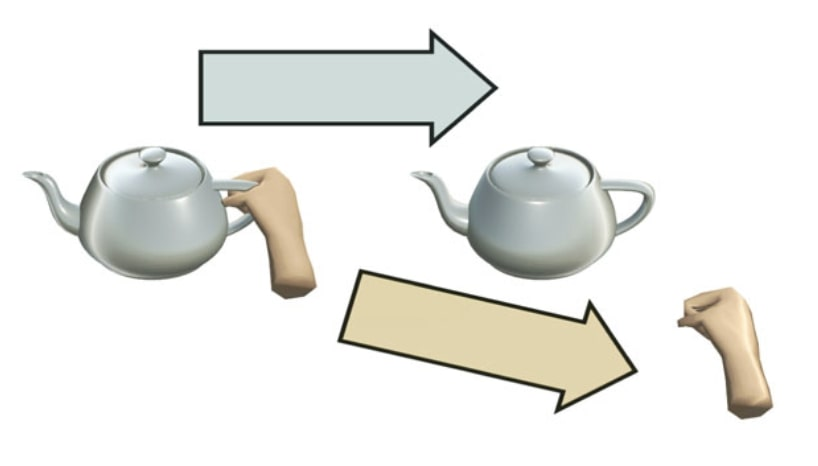
\includegraphics[width=.32\textwidth]{figure/prism.jpg}
    }
    \hspace{2em} % 水平间隔
    \subfigure[Go-Go]{
        \label{fig-1-m}
        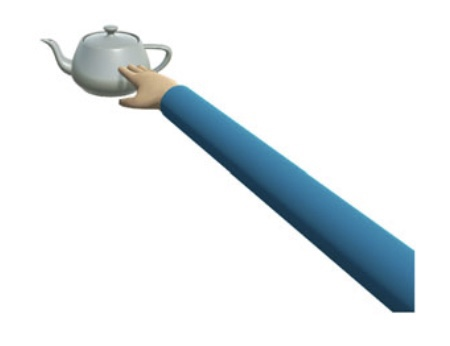
\includegraphics[width=.22\textwidth]{figure/gogo.jpg}
    }
    \hspace{2em} % 水平间隔
    \subfigure[射线广播]{
        \label{fig-1-r}
        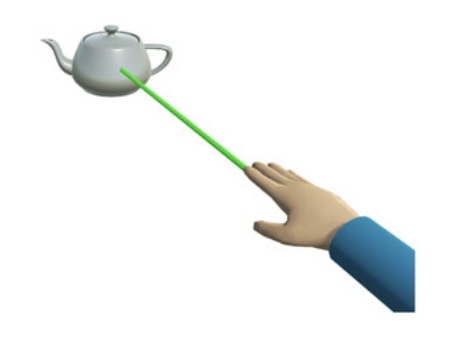
\includegraphics[width=.22\textwidth]{figure/raycasting.jpg}
    }
    \caption{研究早期三种主要的基于手部动作追踪的对象操纵方法}
    \label{fig-1}
\end{figure}

在基于手部(含手柄)追踪的方法研究早期,学界主要的三大思路为在虚拟环境中单手直接操纵、延长用户手臂和射线广播(ray-casting),见图\ref{fig-1}。虚拟延长手臂思路的代表研究来自于Ivan Poupyrev团队在1996年发表的Go-Go沉浸式交互方法\upcite{1996Poupyrev}。Go-Go使用交互式增长用户手臂的元函数和非线性映射来指定和操纵远处的物体。与同时期的其他技术不同的是,Go-Go允许对附近的和远处的物体进行无缝直接操纵。然而,Go-Go技术提出的物体选择和操控模式并不能完全作为一个完整的交互方法来供人们使用; Go-Go应该被视为以同时期技术为基础的一个补充,而不能完全取而代之。射线广播的思路和虚拟延长手臂类似;射线广播的思路是将射线束从使用者的手中延伸出来,从而指定操纵物体。然而,射线广播思路存在比较明显的弊端。由于在射线广播的对象操纵中物体是被连接到射线末端的,所以除了以射线本身为轴可以完成的动作,许多操纵都是难以简单实现的,因为只有一个自由度(围绕射线轴的旋转)可以用射线广播的方式独立控制。比如,若用户希望以与射线方向垂直的轴向旋转一个物体,单纯以射线广播是无法完成的。此外,射线广播还缺乏一种控制物体与用户之间距离的方法,导致用户无法准确地将物体拉近或推远,而这也是对象操纵的基础功能之一。

当把Go-Go方法和射线广播以及其他方法(例如通过将虚拟手臂延伸到无限远来改进Go-Go的Stretch Go-Go)进行比较时,并没有明显的赢家\upcite{1997Doug}。用户评估结果显示,所有技术都有明显的缺点。在这次评估中,HOMER方法被提出来了;这是一种以手为中心的基于射线广播的对象操作技术\upcite{1997Doug}。HOMER使用射线来选择物体,在选择物体后,它将虚拟的手移动到物体上;用户的身体和手之间的当前距离被映射为到虚拟物体的距离。因此,HOMER方法操纵对象的方式与Go-Go技术类似,但缩放系数是针对每个选定的物体独立计算的。

\begin{figure}[t!]
    \centering
    \subfigure[基于双手直接操纵的Z技术]{
        \label{fig-2-u}
        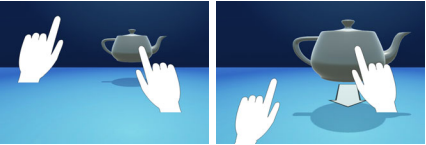
\includegraphics[width=.45\textwidth]{figure/z_technique.png}
    }
    \subfigure[基于双手直接操纵的Sticky Tools方法]{
        \label{fig-2-d}
        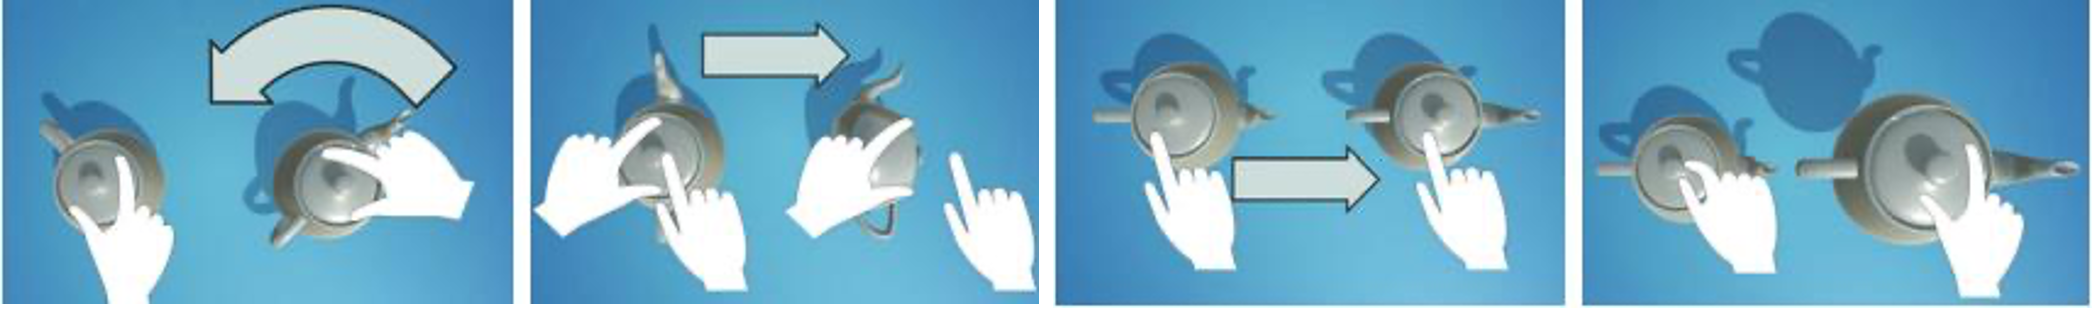
\includegraphics[width=.9\textwidth]{figure/sticky.png}
    }
    \caption{两种具代表性的基于双手动作的对象操纵方法}
    \label{fig-2}
\end{figure}

到了21世纪,学界将研究重心放在虚拟环境对象操纵的精确性上。一个具有代表性的方法是Scott Frees团队在2005年提出的PRISM\upcite{2005Frees},(见图\ref{fig-1-l})PRISM是一种通过缩放操作进行精确和快速交互的方法,它在同时期是一种非常新颖且具有开创性的交互技术。PRISM主动根据用户在虚拟环境中的行为特征来确定他们所想的操纵目标是明确还是不明确的。当操纵目标明确时,PRISM动态地调整“控制/显示”比例来提高对象操纵的精确度。该比例决定了物理手部运动和受控虚拟物体运动之间的关系,降低了传感器对手部运动监测不必要的灵敏度,从而减少操作误差。使用PRISM,用户始终完全控制着被操纵物体的位置。与像Go-Go这样的技术相比,PRISM在能力范围上也有很大提升,最明显的进步在于PRISM扩大了手部运动的规模以允许“远距离”操纵,同时在特定情形中可以主动缩小手部运动的幅度以提高精确度。

在这之后,Curtis Wilkes等人将PRISM与HOMER相结合,在2008年提出了融合了两种方法精华的Scaled HOMER\cite{2008Curtis}。Scaled HOMER使用基于速度的缩放,允许用户在近距离和远距离进行更为精确的操作。它比原始的HOMER在各种任务条件下,尤其是有关需要高度精确、远距离放置物体或大运动距离的任务中的性能都有所提高。2015年,在Go-Go和PRISM研究之后,Chris Auteri等人将这两种技术结合起来,以提高延伸的三维操作的精确性\upcite{2015Auteri}。该方法首先将PRISM直接应用于用户的手(基础光标)的运动,从而基于运动速度计算出一个新的光标位置(PRISM光标)。然后,PRISM光标移动的距离被基于Go-Go距离的启发式方法所放大。与 PRISM和HOMER的结合一样,Go-Go和PRISM的结合提供了一些改进,尤其是在任务完成的成功率和精细度上。

\begin{figure}[t!]
    \centering
    \subfigure[Houde团队的方法]{
        \label{fig-3-l}
        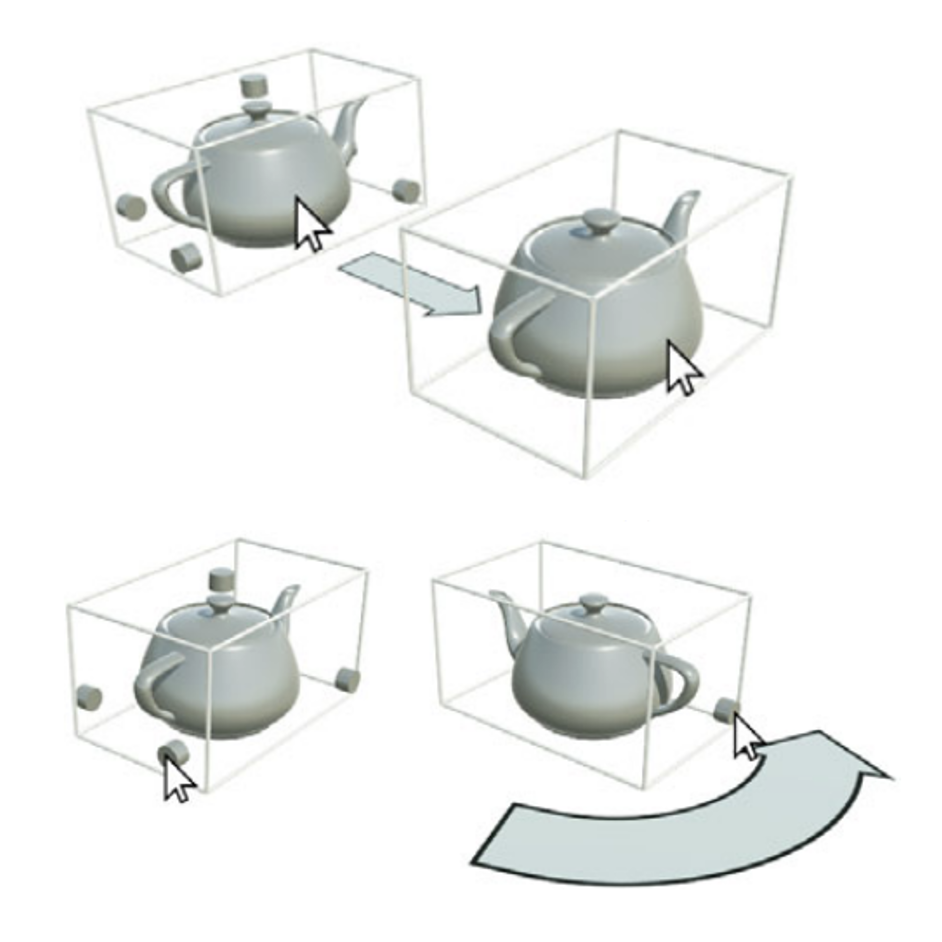
\includegraphics[width=.38\textwidth]{figure/handle_box.png}
    }
    \hspace{5em} % 水平间隔
    \subfigure[Conner团队的方法]{
        \label{fig-3-r}
        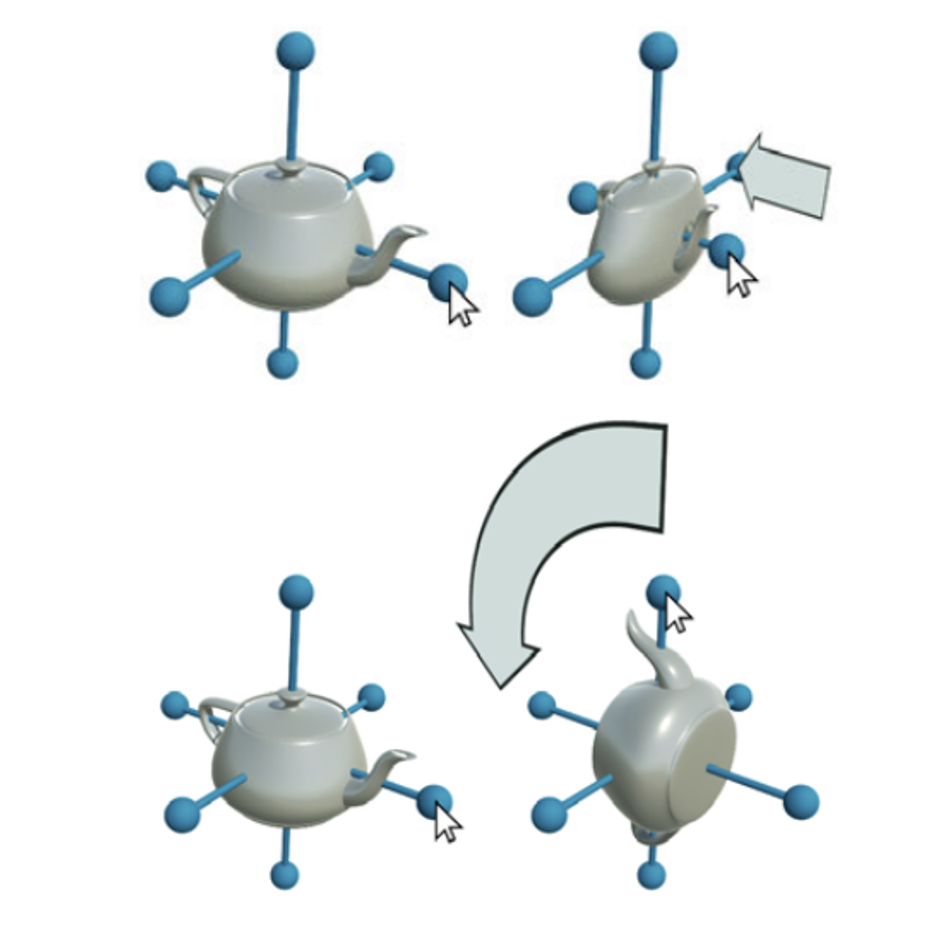
\includegraphics[width=.38\textwidth]{figure/virtual_handles.png}
    }
    \caption{两种具代表性的基于外加虚拟控制柄的对象操纵方法}
    \label{fig-3}
\end{figure}

基于双手的操纵在2008年被Noritaka Osawa团队提出\upcite{2008Noritaka}。该团队提出了一种用于在沉浸式虚拟环境中精确定位3D虚拟物体的单手和双手控制技术。这个方法提出了一种位置调整策略,包括一个类似于PRISM的用于减缓手部运动的比例系数以及一个被动的视角调整。该交互系统会自动将视角接近抓取点,使被操纵的物体看起来更大,从而更易于操控。为了有效控制这些调整,该团队提出了两种技术。第一种是基于单手操纵的;因为当用户想精确地操纵一个物体时,他们的手会慢慢移动,所以通过对单手的速度监测,系统可以判断当前对象是否需要精确操纵。另一种是基于两手间距离的;当用户两手之间的距离很小时,调整就会被激活。通过用户评估,位置和视点的调整比禁用这种调整有更好的操纵效率和用户体验。此外,该团队的测试结果还显示,双手控制比单手表现更好。承接双手直接操纵的方法,Martinet团队提出了两种移动3D对象的技术\upcite{2010Martinet}。第一种扩展了许多CAD(Computer-aided Design,计算机辅助设计)应用程序中的视窗概念;它引入了四个视窗,每个视窗显示3D对象的不同视图。在其中一个视窗中触摸并拖动物体,可以在与该视窗平行的平面上平移物体。第二种方法被称为Z技术;Z技术只使用场景的一个视图(见图\ref{fig-2-u})。在这种技术中,第一次触摸触发在平行于视图的平面上移动物体,第二次触摸触发垂直于视图平面的前后运动。Martinet的初步评估表明,用户更喜欢Z技术。Martinet等人在Z技术的基础上进行了改进,推出了DS3,一种基于DOF分离的三维对象操纵技术\upcite{2010MartinetDOF}。与Z技术类似,一次直接触摸可以在屏幕平面上移动物体,间接触摸可以操纵物体深度,两次直接触摸可以实现旋转。Martinet将DS3与之前的类似方法,比如Hancock团队提出的Sticky Tools方法(见图\ref{fig-2-d})和Reisman团队提出的Screen-Space方法进行了比较,结果显示DOF分离导致了更好的结果\upcite{2009Hancock}\upcite{2009Reisman}。

\begin{figure}[t!]
    \centering
    \subfigure[LTouchIt]{
        \label{fig-4-l}
        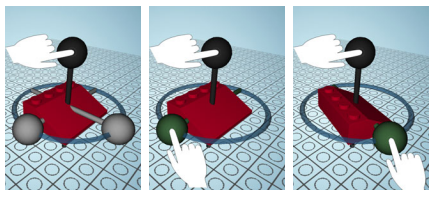
\includegraphics[width=.48\textwidth]{figure/ltouchit.png}
    }
    \hspace{0.2em} % 水平间隔
    \subfigure[多点触控方法]{
        \label{fig-4-r}
        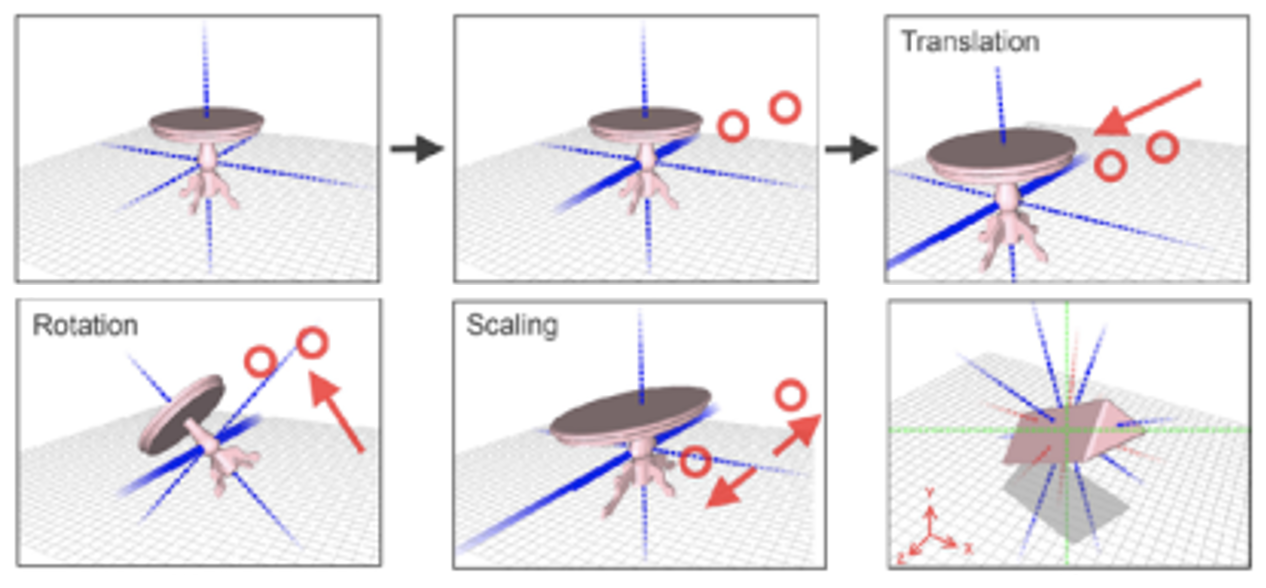
\includegraphics[width=.47\textwidth]{figure/multi_touch.png}
    }
    \caption{两种基于手部动作(含手柄)追踪的非直接对象操纵方法}
    \label{fig-4}
\end{figure}

另外一种值得一提的基于手部动作追踪的方法是外加虚拟控制柄(见图\ref{fig-3});虽然这类方法暂未被应用到虚拟环境中,但是它们对于对象操纵的研究是颇具启发的。Houde团队在1992年开发了一种基于“操纵盒”的方法;这种方法由一个围绕着物体的边界长方体框组成,拖动长方体即拖动物体,另外还有三个旋转柄用于围绕其中心轴旋转物体\upcite{1992Stephanie}。Conner团队也采用了设置虚拟控制柄来进行对象操纵;他们的方法允许完整的9-DOF(Degree of Freedom,自由度)控制(平移、旋转和缩放)甚至诸如扭曲的其他变形\upcite{1992Conner}。该方法的虚拟控制柄的两端有一个小球体,它们将几何变换约束在一个平面或轴上;用户拖动其中一个球体可以平移、旋转或缩放物体。秉承着这两个方法的思想,Mendes团队在2016年提出了相似的一个基于外加虚拟控制柄的方法。他们从实验结果中提出了一套发展准则:(1)直接操作很适合粗略的变换;(2)位移和旋转操作应尽可能分离,以防止不需要的变换;(3)单一的DOF分离对于精确的变换是非常理想的,通常用于细粒度的调整。

2010年以后,基于手部动作(含手柄)追踪的非直接对象操纵方法开始出现。其中较有代表性的两个方法为Mendes团队在2011年提出的LTouchIt和Kin-Chung Au团队在2012年提出的多点触摸方法(见图\ref{fig-4})。LTouchIt虽然使用了直接操纵平移的方法,但在DOF分离之后,它可以控制物体在不超过两个维度上的位置,并使用旋转手柄一次围绕一个轴进行旋转;用户可以选择一个手柄来定义一个旋转轴,并通过另一只手的操作来指定旋转角度\upcite{2011Mendes}。Au团队利用多点触摸表面的高输入带宽,将标准变换部件的操作能力委托给多点触摸手势。这使得使用单一的多点触控动作就能对约束和变换操作进行无缝控制。用户可以用两个触摸点选择一个候选轴,通过按住并移动两个手指来进行物体的变换\upcite{2012Au}。

目前,基于手部动作(含手柄)的追踪的对象操纵方法的SOTA(state-of-the-art,最先进方法)为Gloumeau团队在2020年提出的PinNPivot方法\upcite{2021Gloumeau}。这个方法使用“销钉(pin)”来约束1DOF/2DOF/3DOF旋转;PinNPivot还支持6DOF操纵和3DOF平移,具体的一个操作流程可参考图\ref{fig-5}。在该团队与以往技术的比较表明,PinNPivot拥有更准确和更快的操纵效率。

\begin{figure}[t!]
    \centering
    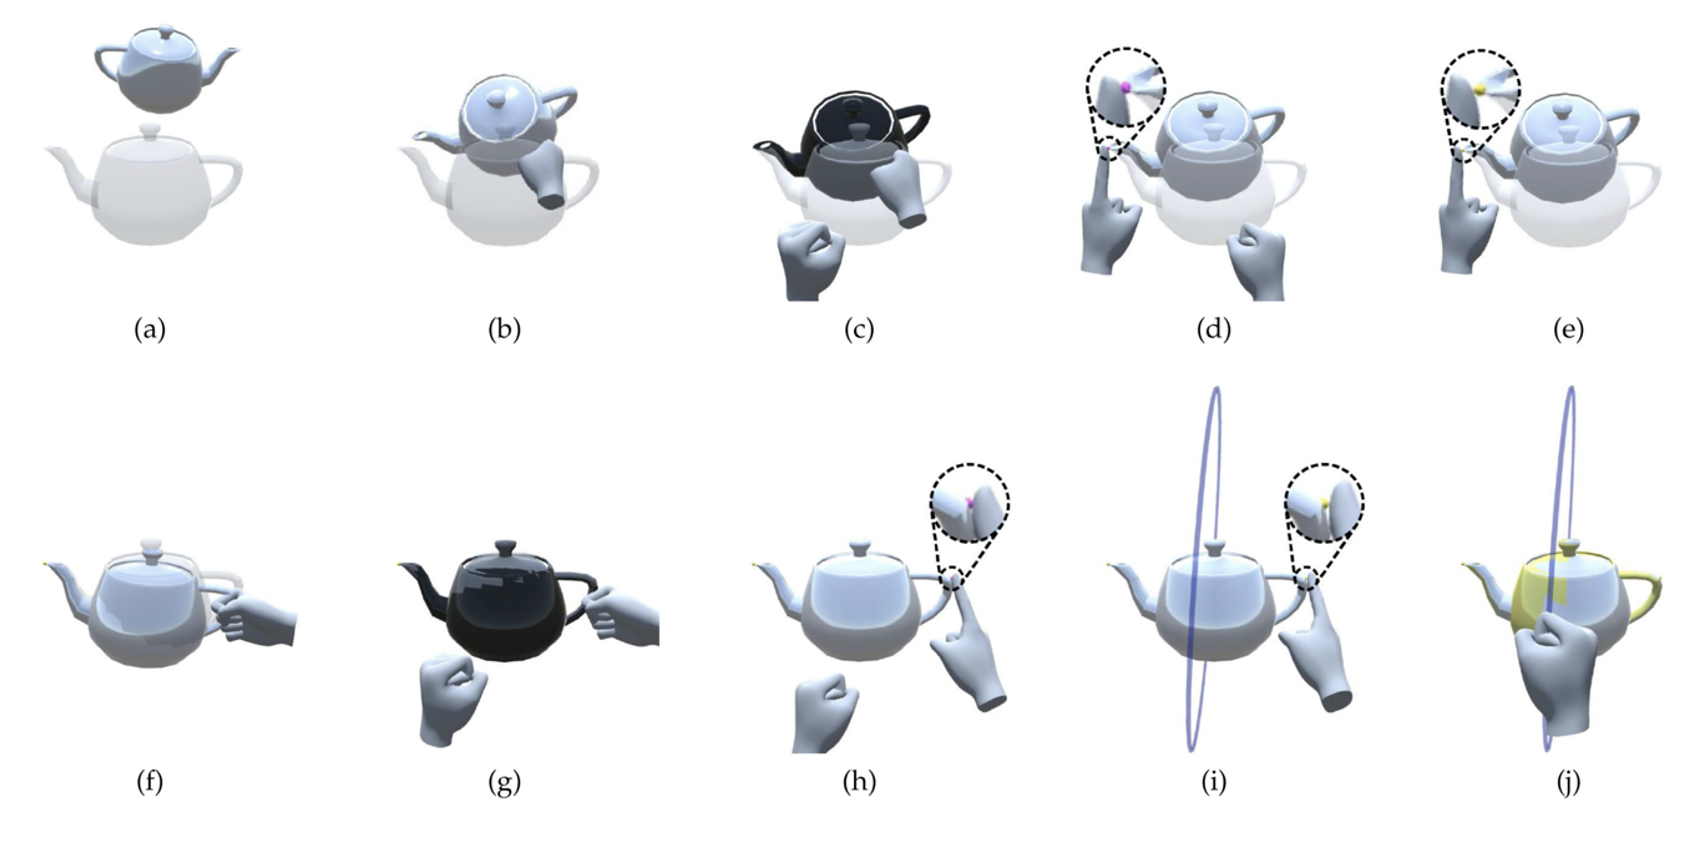
\includegraphics[width=.99\textwidth]{figure/pinnpivot.png}
    \caption{目前基于手部动作(含手柄)的对象操纵最优方法:PinNPivot}
    \label{fig-5}
\end{figure}

\section{基于眼动的操纵}

在2015年以后,眼球追踪在头戴式虚拟现实显示器中的应用越来越多,各种集成了眼球追踪器的头盔已经在市场上销售。根据Adhanom团队在2023年发表的研究,眼动跟踪在虚拟现实中的应用是高度多样化的,并且跨越了多个学科\upcite{2023Adhanom}。因此,近年来基于眼动追踪的对象操纵方法应运兴起。

在VR中实现基于眼睛注视的指向的最常见方法是使用眼动仪提供的3D注视方向向量,并观察场景中的哪些对象与方向向量相交\upcite{2019Sidenmark}。通常,射线是基于方向向量投射的,并且射线相交的第一个物体被认为是被指向的项目(见图\ref{fig-6})。这与射线广播的基本思想是一致的。各种研究表明,基于凝视的指向比基于手的指向更快,因为我们能够比我们的手更快地将目光移向目标\upcite{2000Tanriverdi}。然而,由于眼球运动的固有生理特性和眼动追踪的技术限制,与其他常见的指点界面相比,基于眼睛注视的准确度还是稍显逊色的\upcite{2018Hansen}\upcite{2019Luro}。基于眼睛注视的指向界面中的不准确性主要有两种形式,一是由眼睛跟踪数据中的自然噪声引起的,二是由眼睛跟踪数据质量不稳定引起的。

\begin{figure}[b!]
    \centering
    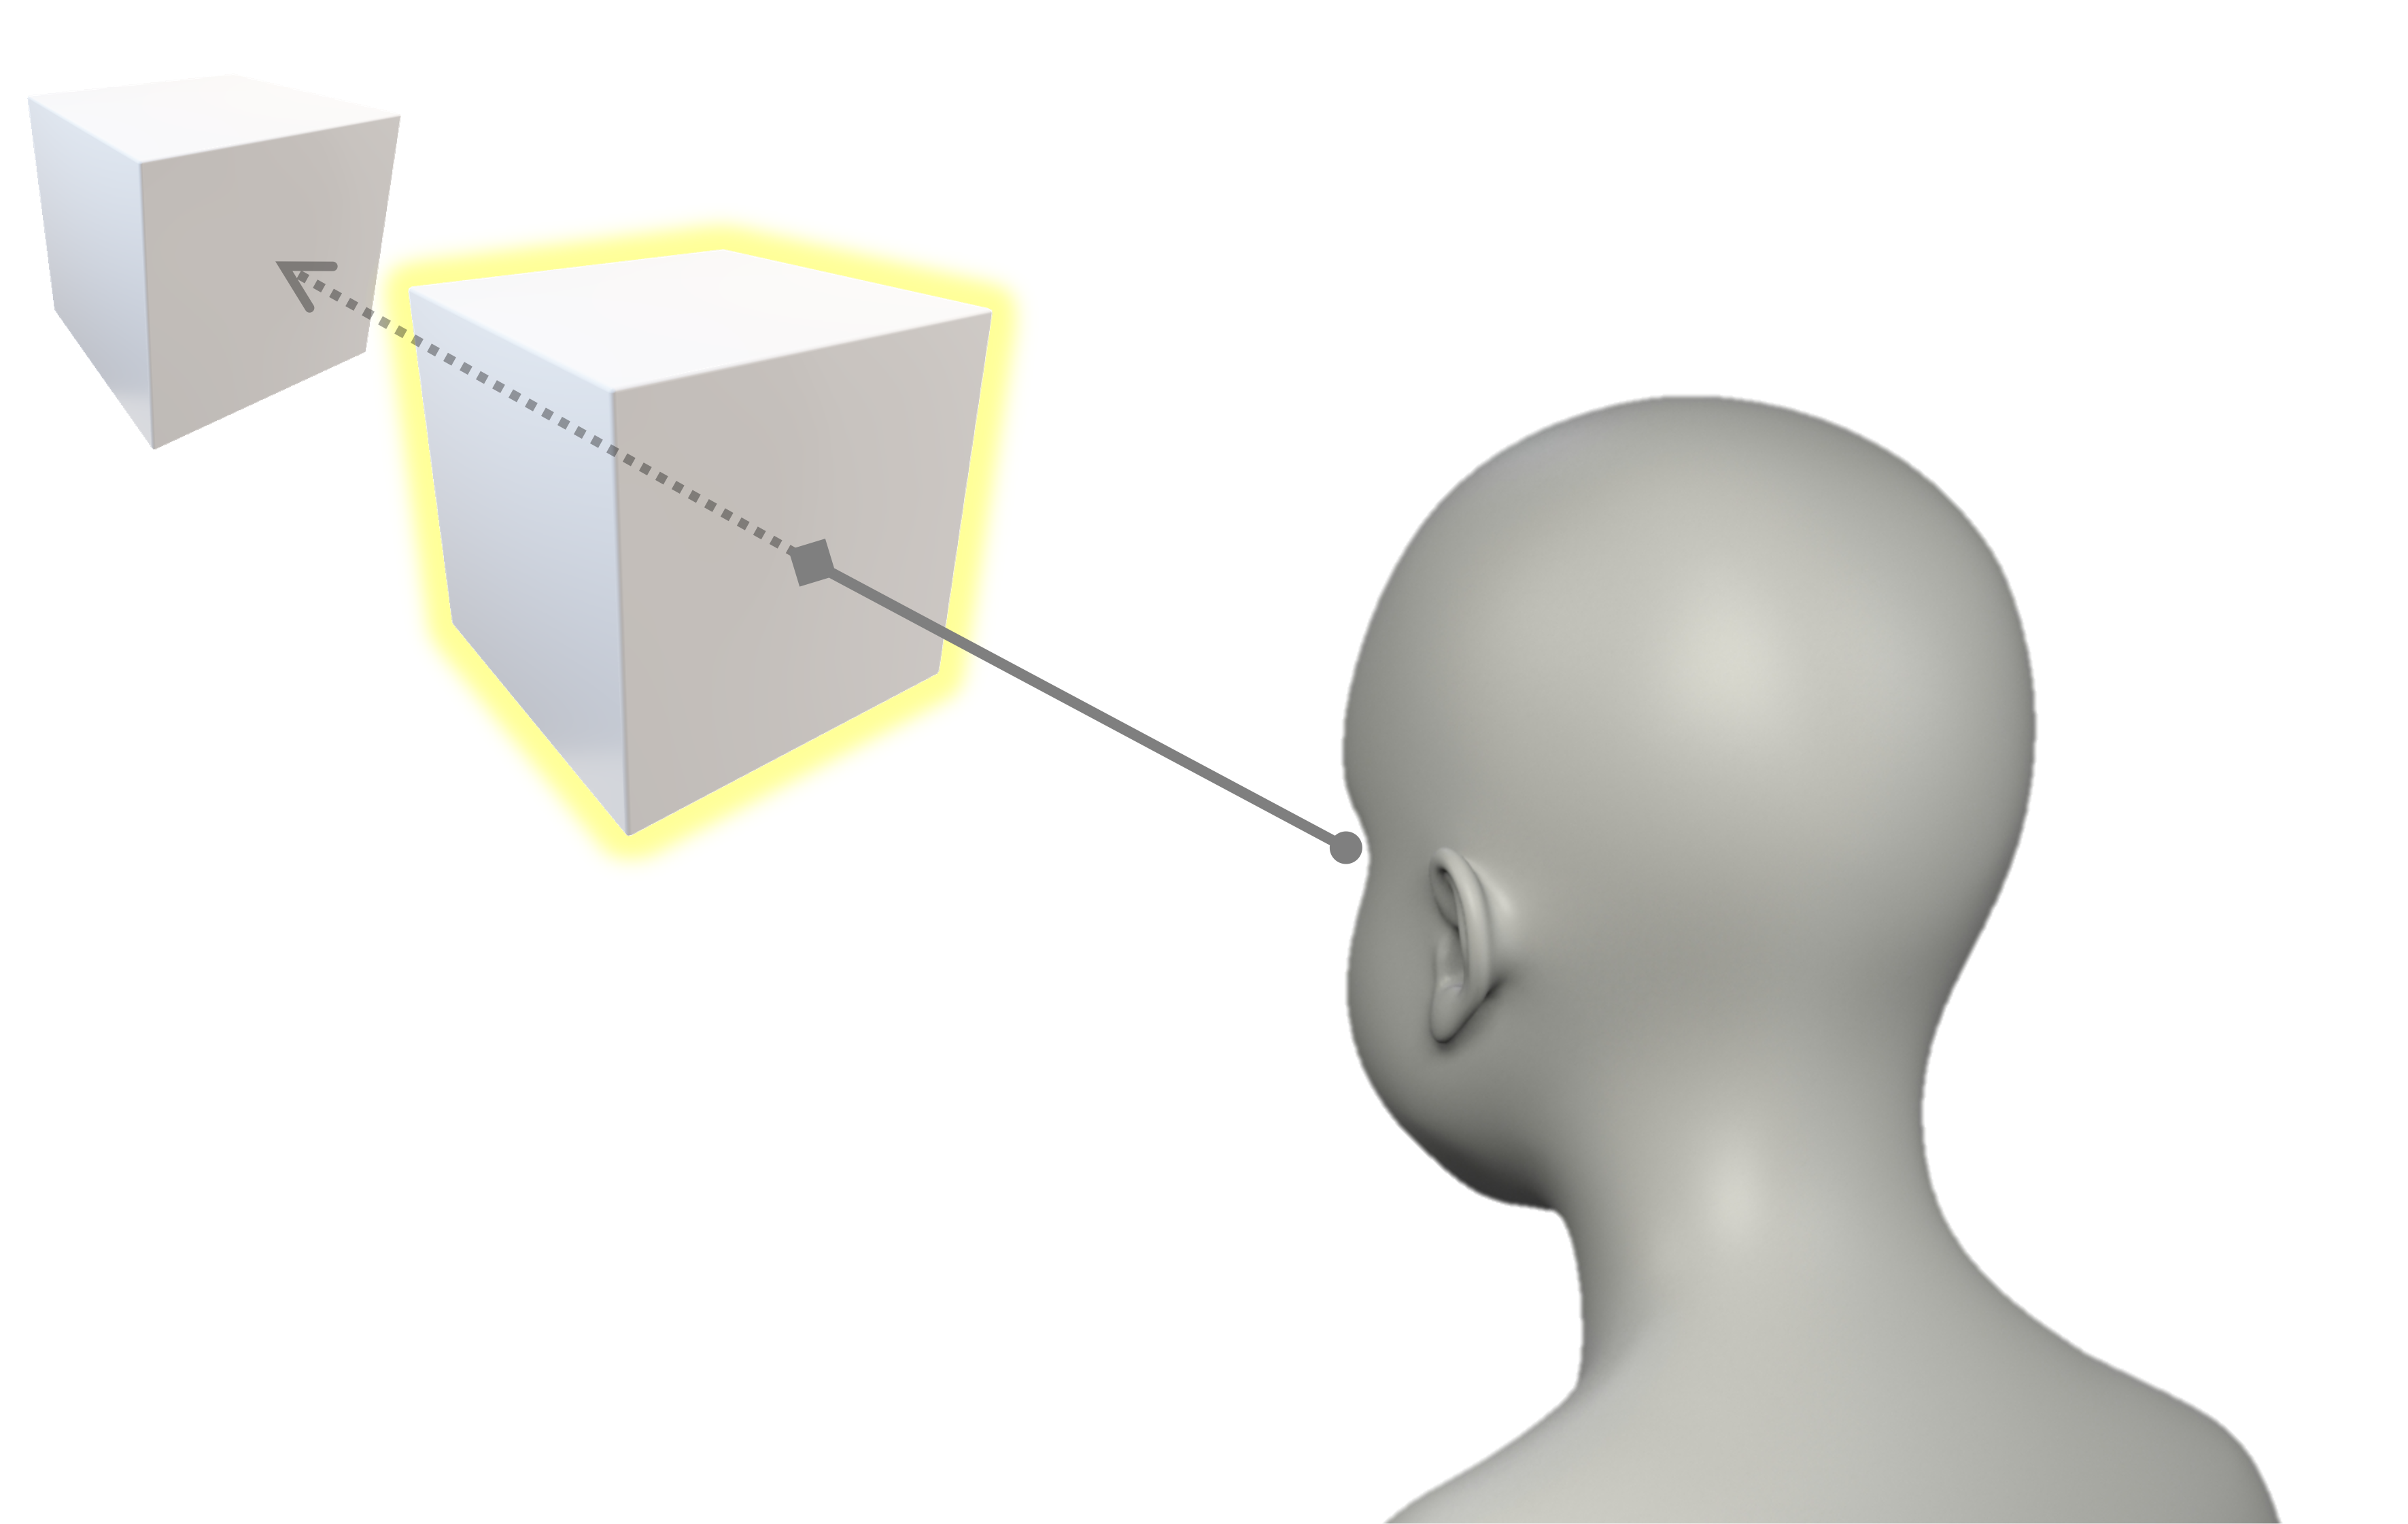
\includegraphics[width=.45\textwidth]{figure/gazing_raycasting.png}
    \caption{基于眼睛注视的指向选择}
    \label{fig-6}
\end{figure}

基于眼动追踪的操纵方法的一大难点是目标对象选择。仅通过眼睛注视进行选择是一项相对具有挑战性的任务,需要实施更为精密的机制以在虚拟环境中使用基于眼睛的交互。根据以往的方法,我们可以实施其他选择确认技术来辅助眼动交互。这样做的一个额外好处是可以解决人机交互领域经典的“点石成金”问题,即“无论你看哪里,都有东西被激活;你不能在没有发出命令的情况下看任何地方”\upcite{1990Jacob}\upcite{2016Jacob}。

\begin{figure}[t!]
    \centering
    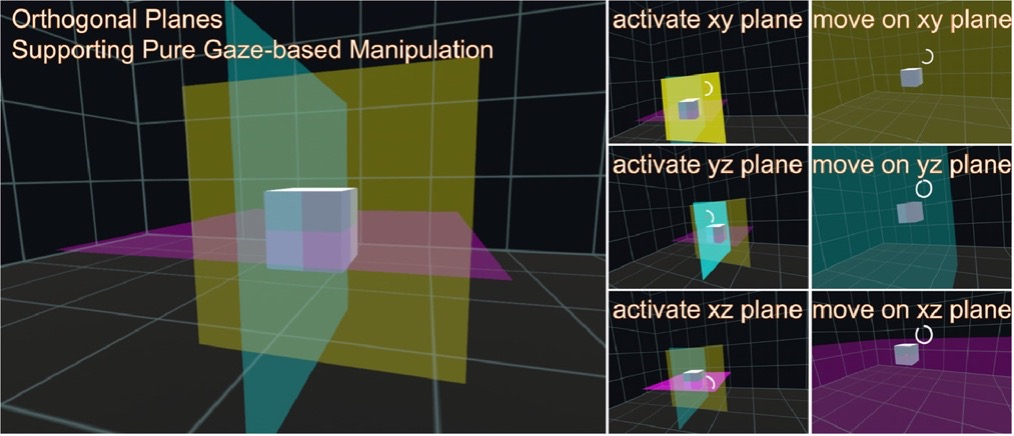
\includegraphics[width=.7\textwidth]{figure/orthogaze.jpg}
    \caption{一个基于眼动和正交平面的对象操纵方法:OrthoGaze}
    \label{fig-7}
\end{figure}

目前已有许多学者使用各种技术来实现虚拟环境中基于注视的交互选择确认。Hansen团队在2018年提出了一种基于眼睛注视的停留进行选择确认的技术\upcite{2018Hansen}。Sidenmark和Gellersen在2019年实施了两种头部辅助的眼动交互技术,第一种是Eye \& Head Dwell,第二种是Eye \& Head Convergence\upcite{2019Sidenmark}。Eye \& Head Dwell是一种停留以确认的技术,其中停留计时器仅由头部支持的凝视转移触发,但可以通过仅眼睛凝视暂停和恢复;Eye \& Head Convergence是一种用于快速目标确认的替代技术,它允许用户通过将眼睛指示器和头部指示器对准目标来确认选择。Kumar和Sharma团队在2016年提出了一种使用眨眼进行选择确认的技术\upcite{2016Kumar}。Pfeuffer团队在2017年提出了一种手眼协统的选择确认方法;这个方法允许用户用眼睛注视物体并同时加以一种“捏合”手势来辅助确认选择\upcite{2017Pfeuffer}。Pai团队在2019年提出了另外一种协同辅助操纵技术;用户可以用目光指向目标,并使用肌电图检测到的手臂肌肉收缩来触发操纵动作\upcite{2019Pai}。Qian和Teather团队在2017年提出了一种通过键盘按钮按下进行选择确认辅助,并使用眼睛注视进行指向选择的方法\upcite{2017Qian}。最近,Sidenmark团队在2020年提出了Outline Pursuits方法,它利用平滑追踪来允许用户在虚拟环境中选择被遮挡的对象\upcite{2020Sidenmark}。

伴随选择技术而来的另外一个值得关注的问题是反馈技术。一个完整的虚拟环境中的对象操纵技术应该向用户提供反馈,让用户能够清楚地了解系统的状态\upcite{2014Majaranta}。由于眼睛对视野中的视觉变化很敏感,它们会本能地尝试将注意力转移到这些视觉变化上。因此,在向用户提供反馈时应该格外小心,因为视觉上突出的反馈机制可能会产生意想不到的后果,即转移用户的视线以产生不期望的交互动作。Boyer团队在2017年提出的一种非视觉反馈方法,他们使用听觉反馈来避免不必要的视线转移\upcite{2017Boyer}。然而,学界依然有很多基于视觉的反馈方法:Blattgerste团队在2018年提出了一种突出显示所选对象的反馈方法;Mohan团队也在2018年提出了一种在所选对象周围显示确认标志的方法;Sidenmark团队在2020年提出了一种在所选对象周围显示轮廓的反馈方法\upcite{2018Blattgerste}\upcite{2018Mohan}\upcite{2020Sidenmark}。

根据目前基于眼动追踪的对象操纵方法的研究数量,眼动追踪将很快成为HMD系统不可或缺的一部分。因此,我们预计围绕HMD眼动追踪的研究和开发将在未来几年加速和扩展。然而,目前大部分眼动追踪方法依旧存在许多值得优化的问题。除了硬件限制,交互动作所带来的生理性不适也需要得到改善。大多数基于眼动追踪的操纵方法都包含眨眼命令(包括眨眼、双眼眨眼和眨眼眼球运动)\upcite{2016Kumar}。要求用户改变他们的自然眨眼频率可能会导致用户眼睛疲劳、眼睛干涩和眼睛疲劳\upcite{2020Hirzle}。Kumar和Sharma团队在2016年的研究结果也表明,频繁眨眼和眨眼会导致用户眼睛疲劳\upcite{2016Kumar}。而且,基于眨眼的界面往往不准确,因为下意识的眨眼很难与自然眨眼区分开来,所以系统往往需要用户做出完全下意识的眨眼动作,如快速多次眨眼。然而,长时间眨眼有明显的缺点,例如减慢交互流程并在长时间眨眼期间阻挡用户的视线。因此,基于眼睛注视的系统控制需要在交互动作上做出合理的优化。

目前基于头眼协同的最优方法是Liu团队在2020年提出的OrthoGaze,它允许用户只需用眼睛凝视就能直观地操纵虚拟物体的三维位置(见图\ref{fig-7})\upcite{2020Chang}。该方法利用了三个可选择的正交平面,其中每个平面不仅有助于引导用户在任意虚拟空间中的注视,而且还允许对物体位置进行2DOF操作,是一种完全不依赖手部的对象操纵方法。然而,这个方法仅实现了空间位移,而没有考虑旋转和缩放,所以并不能被视为一个完整的操纵方法。

\begin{figure}[t!]
    \centering
    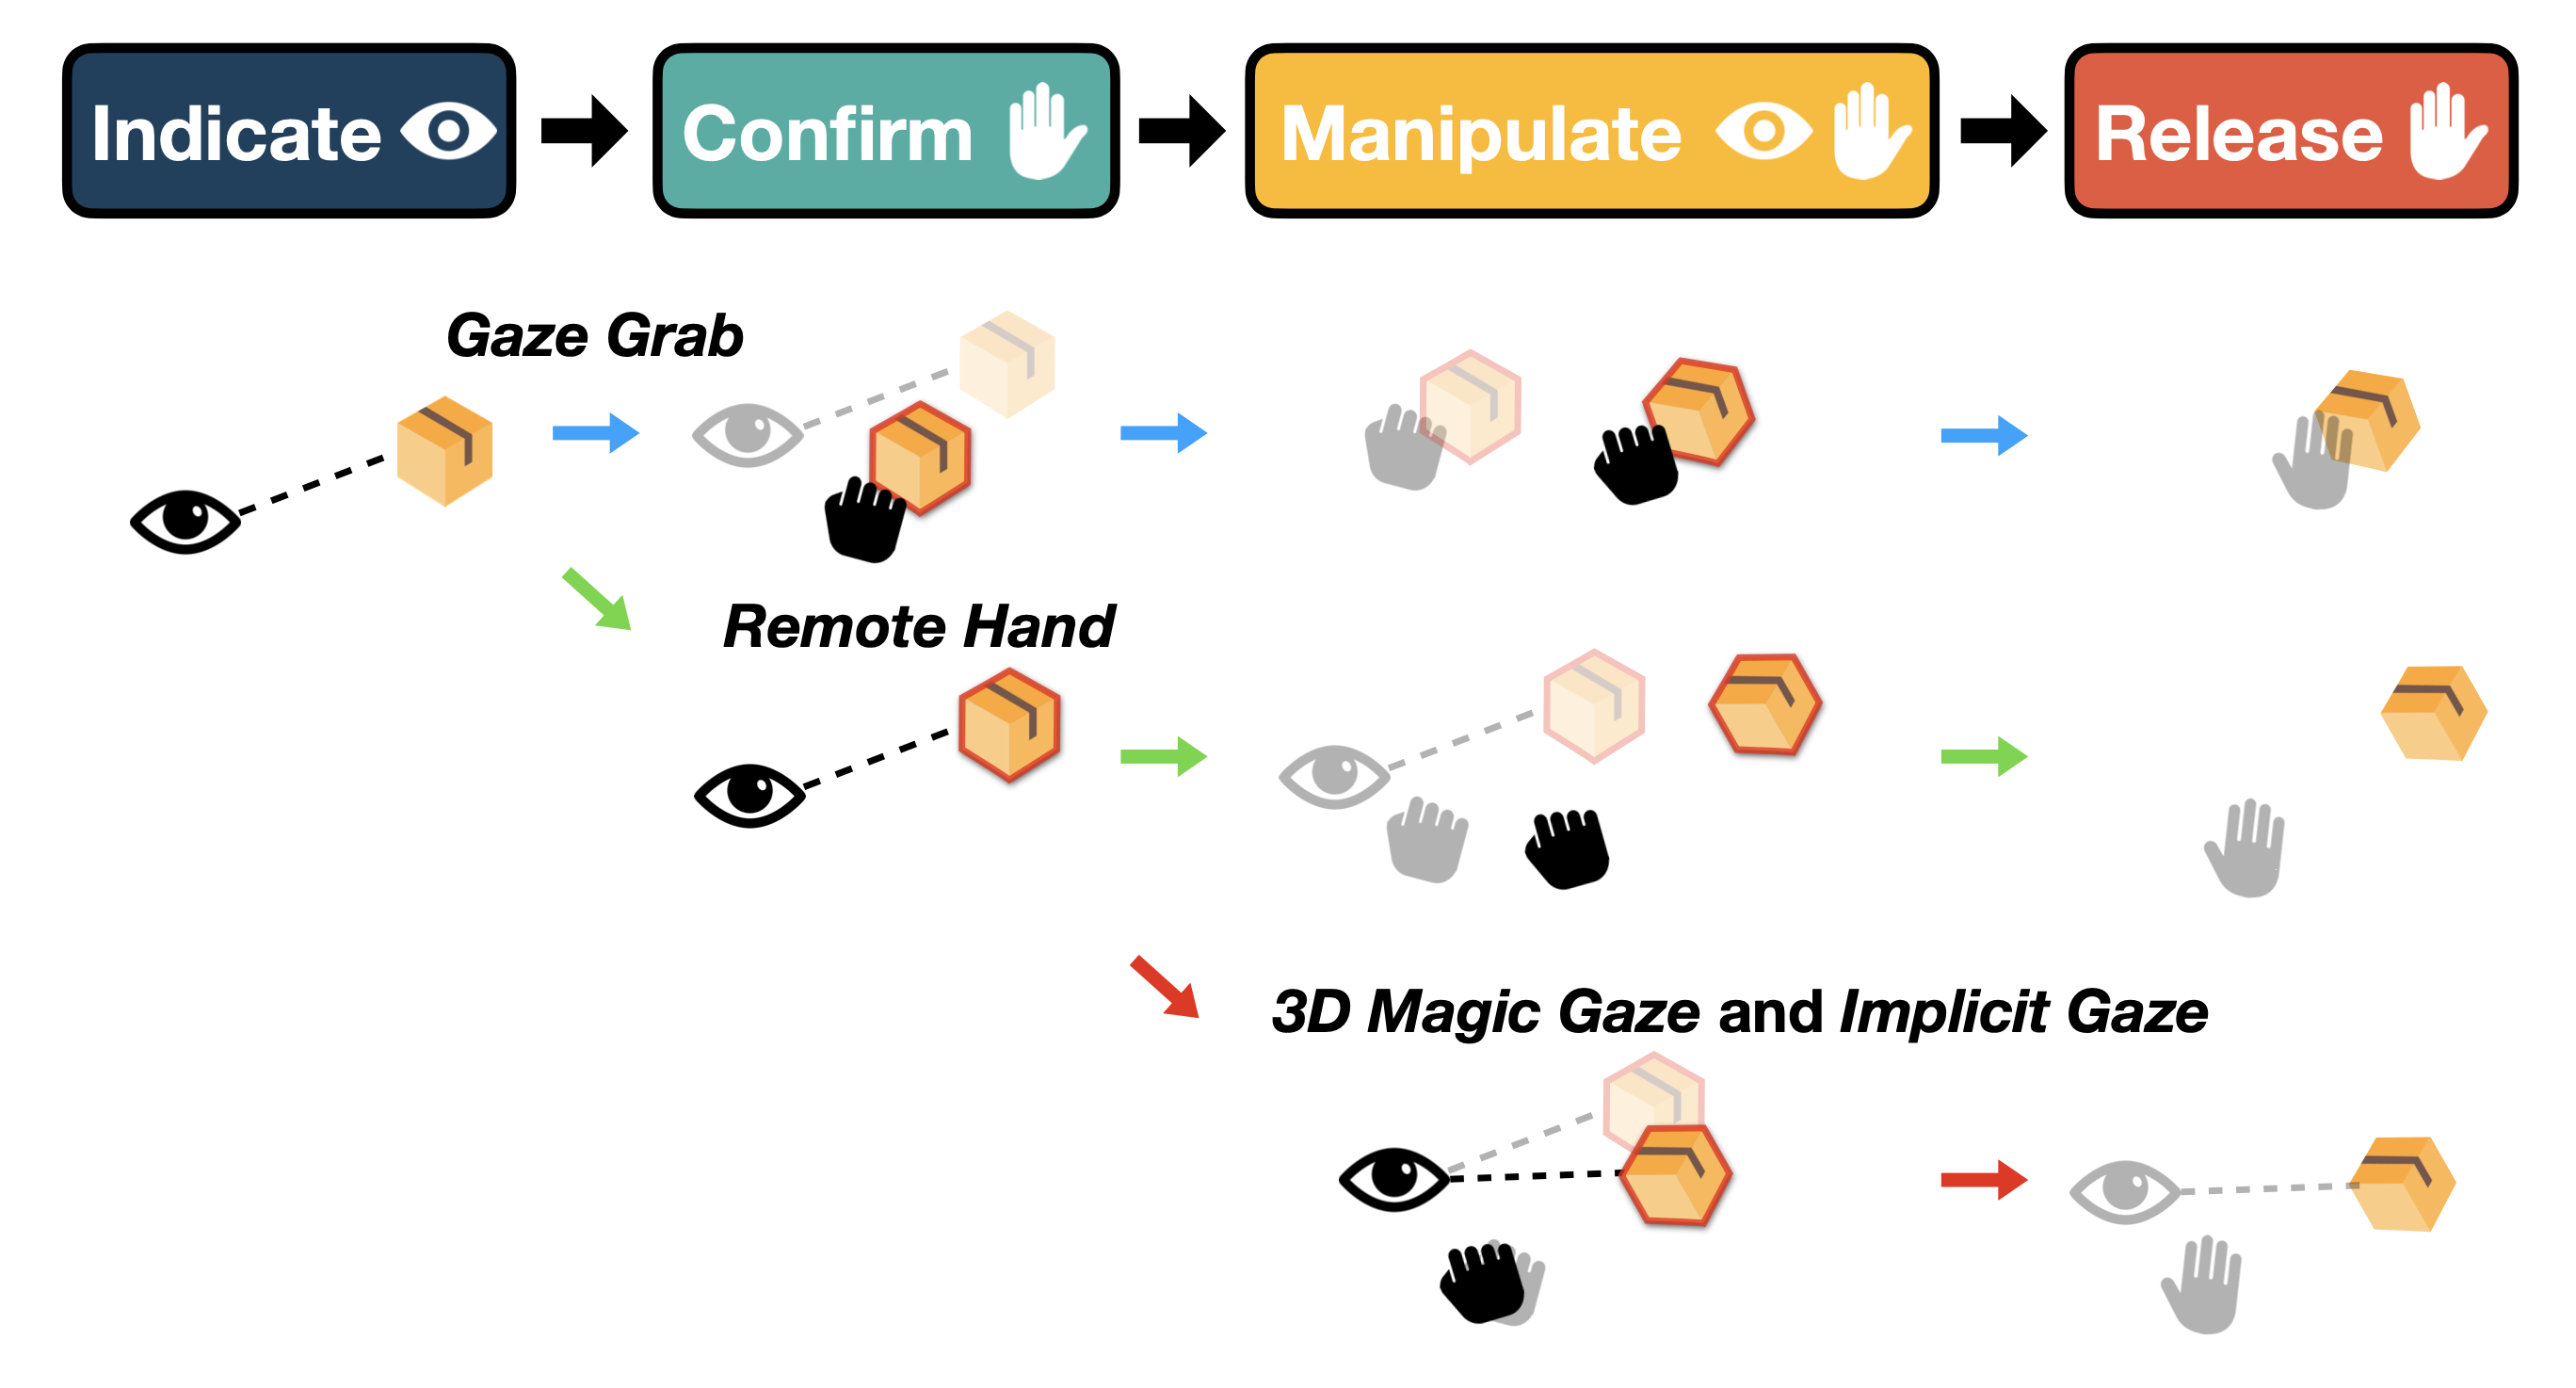
\includegraphics[width=.7\textwidth]{figure/gaze_supported_sota.png}
    \caption{目前涵盖凝视的物体操纵最优方法}
    \label{fig-8}
\end{figure}

目前涵盖眼动追踪的对象操纵方法的最优方法为Yu团队在2021年提出的一种基于凝视和手部动作的三维物体操纵方法Implicit Gaze\upcite{2021Yu}。该方法的整个操纵任务可以分解为四个阶段:指示、确认、操作和释放(见图\ref{fig-8})。该研究表明,当所有目标都位于用户前方且在手臂可触及的距离内时,基于凝视的交互对于物体操作没有明显的性能优势;但对于有远处物体的较大空间,凝视输入可以减轻手臂的疲劳问题。眼动和其他模态的不同整合、协调和过渡策略可以为构建更高效的物体操纵技术提供优势。然而,这个方法依旧依靠手部动作,并不能被视为一个完全无手(hands-free)的操纵方法。

% !Mode:: "TeX:UTF-8"

\chapter{方法设计与实现}

\section{方法概述(Pipeline)}

该对象操纵交互系统的方法流程可以用一个有限状态机来表示,见图\ref{fig-3-1}。

\begin{figure}[b!]
    \centering
    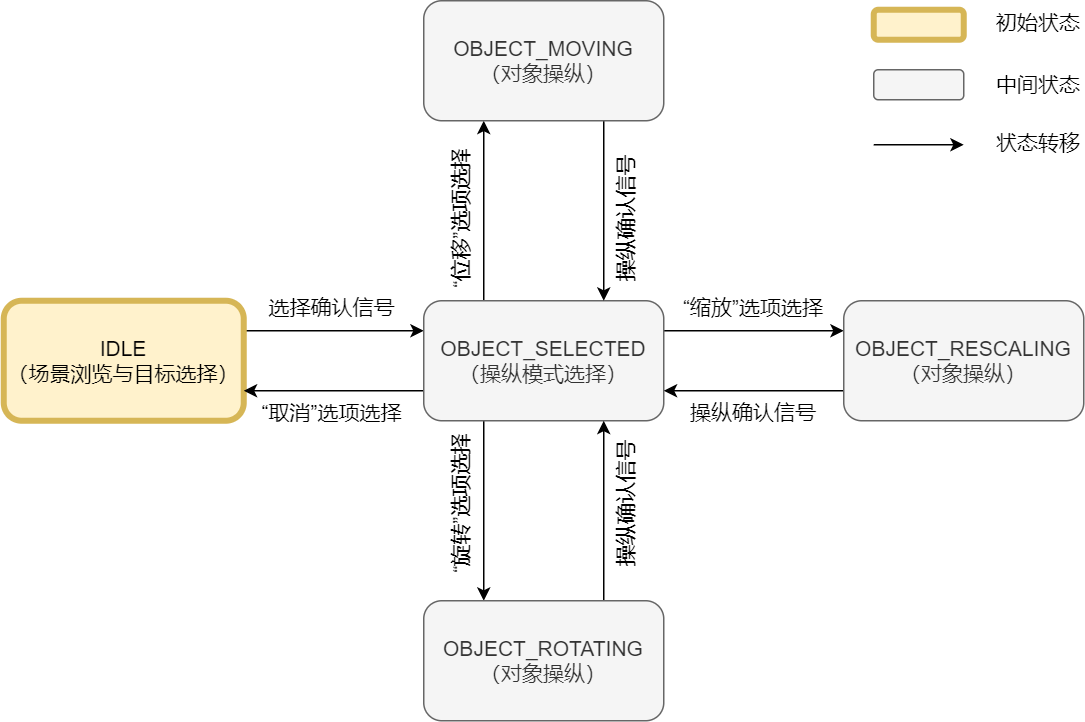
\includegraphics[width=.85\textwidth]{figure/system_state_machine.png}
    \caption{交互系统有限状态机}
    \label{fig-3-1}
\end{figure}

{\bf 场景浏览与目标选择}:对应状态IDLE。在进行目标选择时,用户先以通过头部向前射线指向目标操纵对象,之后以快速两次眨眼作为确认信号选择该对象,该选择和确认方法的优势由Yuan Yuan Qian团队在2017年作过探讨\upcite{yuanyuan2017}。接收到选择确认信号后,进入下一状态;

{\bf 操纵模式选择}:对应状态OBJECT\us SELECTED。生成一个“四叶草”模式选择菜单,用户可以通过凝视某一选项以进入对应的操纵模式,用户也可以通过凝视“返回”选项以退回到1(详见\autoref{Clover});

{\bf 对象操纵}:对应状态OBJECT\us MOVING、OBJECT\us ROTATING或OBJECT\us RESCALING。我们提出的操纵系统支持六自由度(6DOF)操纵。在不同的对象操纵模式下,用户可以对物体进行三自由度位移、二自由度旋转和一自由度缩放(详见\autoref{Manipulation});

{\bf 确认操纵结果}:对应状态转移条件“操纵确认信号”。通过快速两次眨眼作为确认信号以确认当前操纵状态,回到OBJECT\us SELECETD。

\section{场景浏览与目标选择}

该交互系统的浏览和选择方法不需要使用复杂的手柄或其他输入设备,使得用户能够更加自然地与虚拟环境进行交互。

\subsection{场景浏览}

在场景浏览时,该系统通过跟踪用户的头部向前(forward)射线控制场景中虚拟摄像头的移动,将其实时拍摄的场景画面即时反馈到用户的头戴式显示器中,以提供一个自然、直观的场景浏览体验。

其次,我们需要计算实时视点。视点的计算涉及到两个方面:视角和视位。视角是指用户在虚拟环境中的观察方向,通常由头部的旋转角度决定。视位是指用户在虚拟环境中的位置,通常由身体的移动或手柄的操作决定。为了实时地获取用户的视角和视位,需要使用一些传感器或追踪器,例如红外摄像头等。这些设备可以测量用户头部或身体的运动数据,并将其传输给计算机。根据用户的视角和视位,我们可以获取用户当前所期望观察、选中以及操作的物体。

在判断驻留点时,我们使用射线广播(ray-casting)的方法。射线广播是一种在虚拟现实中选择对象的常用技术;在我们的交互系统中,它利用用户的头部向前方向来发射一条射线,与场景中的对象进行碰撞检测,从而获取驻留点。射线广播的优点是简单、直观、高效、学习成本低并且不容易产生眩晕感和迷惑感。当驻留点在某个物体上时,该物体将被高亮,以消除对象选择时的歧义。同时,系统会在用户界面上与头部向前射线相交处生成一个瞄准点,帮助用户瞄准目标对象;该瞄准点仅会在IDLE状态下生成。当目标对象被瞄准后,用户可以通过快速两次眨眼来确认选择。

\subsection{目标选择}

在IDLE状态下,用户可以使用眼动确认信号来选择目标。该部分的主要挑战包括如何准确地捕捉并且解析用户的眼动数据以及如何提供合适的反馈和提示。

最为常见且自然的主动眼动信号有单眼眨眼和快速两次眨眼,因此我们将这两种眼动行为作为我们的最终眼动信号候选池。我们设计了一个前导实验(Pilot Study),目的是从这两种眼动信号中,确定一个最为高效并且带来最小使用压力的眼动确认信号,这将在之后的实验设计章节中作更细致的介绍。通过加权分析两种眼动行为的实验结果,我们最终确定使用快速两次眨眼来作为我们的目标选择以及确认信号。

在选择确认后,系统的状态转移到OBJECT\us SELECTED,并且会提供给用户一个基于听觉的声音反馈信号。这个反馈信号相对于视觉是异模态的,目的是提高交互系统的可靠性以及降低用户的迷惑感。

\section{“四叶草”模式选择菜单}\label{Clover}

\subsection{设计理念}

\begin{figure}[t!]
    \centering
    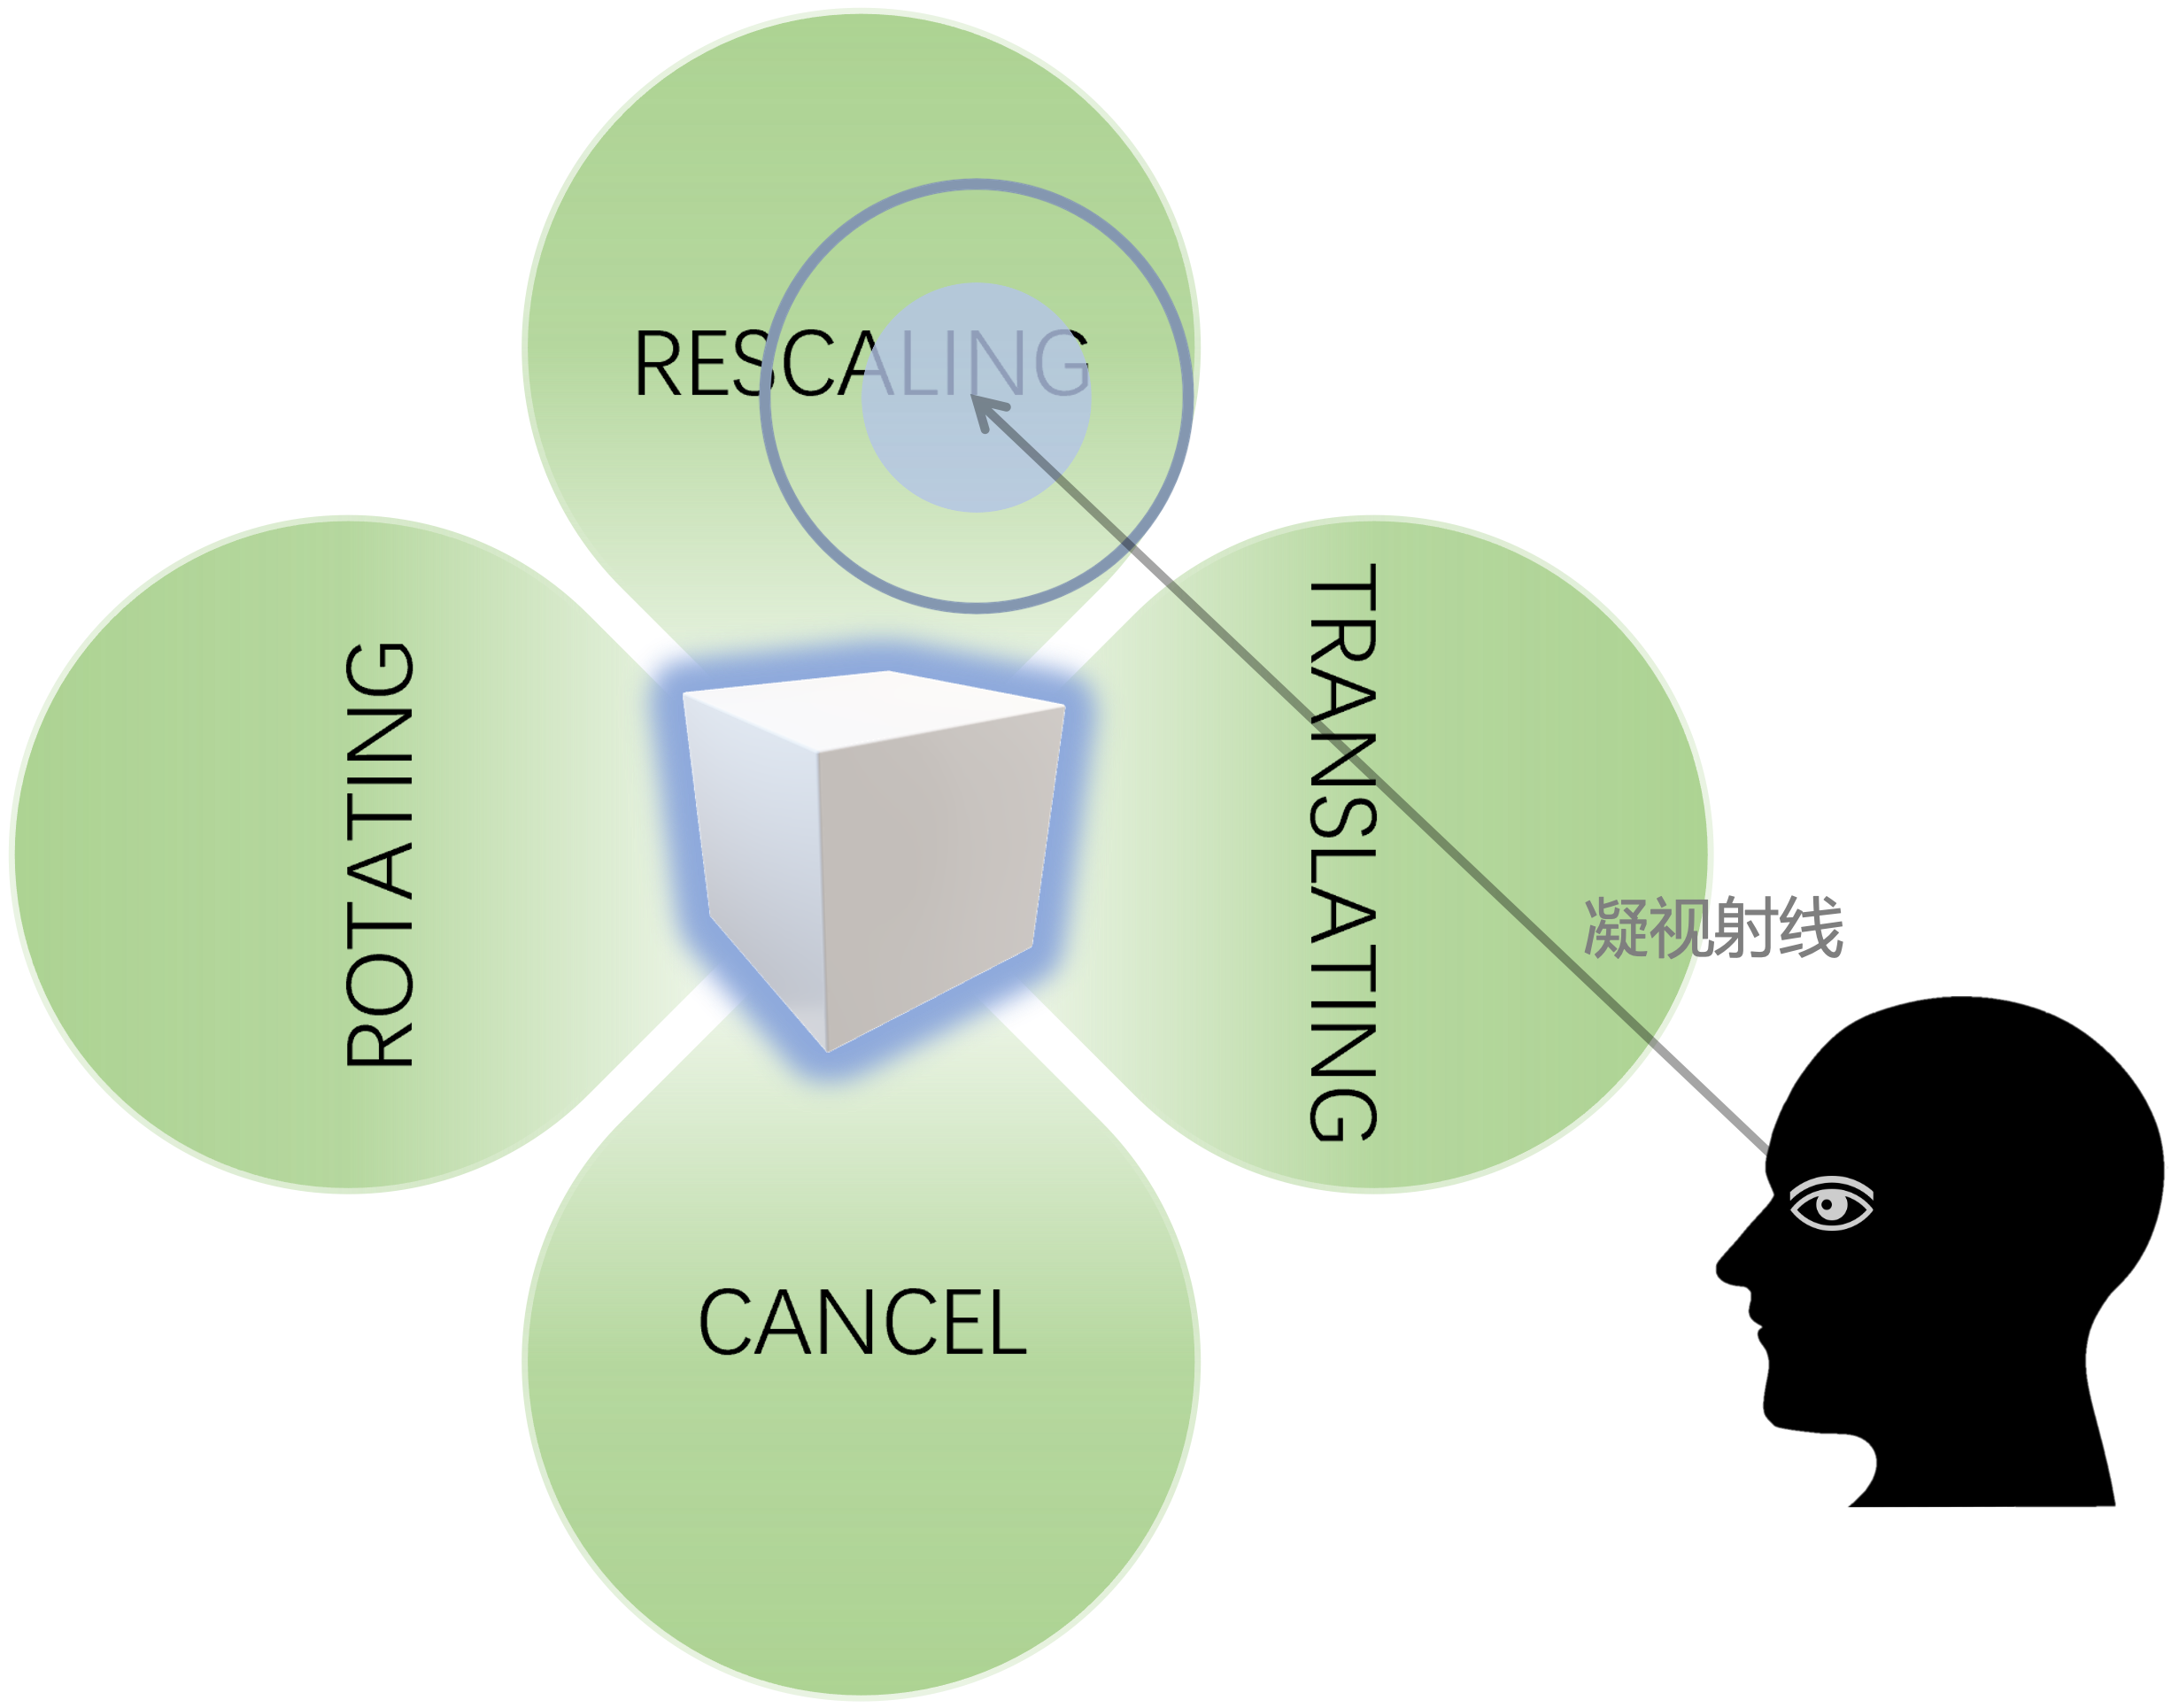
\includegraphics[width=.55\textwidth]{figure/clover.png}
    \caption{“四叶草”模式选择菜单以及选择确认进度盘}
    \label{fig-3-4}
\end{figure}

我们在交互系统设计阶段考虑到大多数实际的完整操纵流程往往不仅包含一个特定操纵模式的选择,还会包含多种操纵模式之间的切换。然而,当前的基于凝视和眼动的交互方法并没有考虑便捷的模式切换;在这些方法中,如果用户需要在一次操纵结束后切换到下一种操纵模式,则需要退回到最初态重新进行一遍从选择到操纵到流程,引入大量冗杂操纵和效率浪费。所以基于此考虑,我们设计了一个“四叶草”模式选择菜单。

我们希望“四叶草”模式选择菜单可以让用户简便地用凝视动作来选择进入或者切换到某种交互状态。

\subsection{菜单说明}

“四叶草”模式选择菜单在且仅在系统有限状态机的OBJECT\us SELECTED状态下生成在用户界面上,用户可以通过它来选择进入到某具体的交互模式:空间位移、空间旋转和空间等比例缩放,分别对应系统有限状态机中的OBJECT\us MOVING、OBJECT\us ROTATING和OBJECT\us RESCALING三个状态;用户也可以通过它来取消选中物体以回到IDLE态。这个过程可以在我们规定的系统有限状态机中体现\ref{fig-3-1}。

菜单在四个方向提供了四个的选项,分别为位移、旋转、缩放和取消;用户可以通过看向相应的方向来选择对应的选项。在规定每个方位具体对应哪个选项时,我们首先设置了一个问卷调查,发放给30个随机人员采样以获取用户根据推测对四个选项使用频率的排序;其次,我们参考Maxwell等人在2006年发表的结论(眼球水平运动的负担比垂直运动的负担小\upcite{2006Maxwell}),将问卷调查中显示最频繁使用的两种交互模式选项(位移、旋转)设置在左右两侧,将剩下的两种选项(等比缩放、取消)设置在上下两侧。

\begin{figure}[b!]
    \centering
    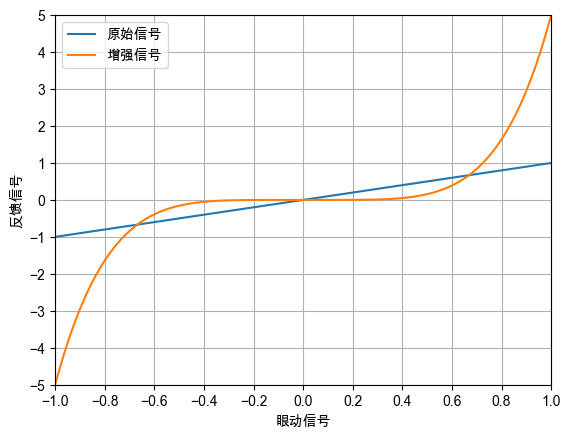
\includegraphics[width=.7\textwidth]{figure/augmented.png}
    \caption{信号增强函数}
    \label{fig-3-2}
\end{figure}

为了避免误触和“点石成金”的人机交互领域经典问题\upcite{2016Jacob},我们规定了一个选择确认时间;该时间默认为1秒,用户也可以根据自己的习惯调整时长。当用户选择时,界面上会显示一个选择确认进度盘(见图\ref{fig-3-4}),此时开始选择确认倒计时;进度盘会随着用户凝视射线持续指向选项而逐渐变满,用户可以在进度盘进度未满之前通过使视线复位来取消选择。当选择确认倒计时结束时,进度盘进度满,用户立即转移至凝视射线指向选项的对应状态。

\section{对象操纵}\label{Manipulation}

我们的交互系统支持完全6DOF的对象操纵,允许用户对目标对象进行空间位移、空间旋转、等比例缩放三种具体的操纵,分别对应系统有限状态机中的OBJECT\us TRANSLATING、OBJECT\us ROTATING和OBJECT\us RESCALING。

在每种对象操纵模式下,我们引入了一种特殊的信号增强函数:

\begin{equation}
	\label{formula-3-1}
	A(v) = 5v^{5}, -1 \le v \le 1
\end{equation}

让用户在小幅度动作时可以对对象进行微调,在大幅度动作时可以让对象作快速动作;其增强效果见图\ref{fig-3-2}。


\begin{figure}[t!]
    \centering
    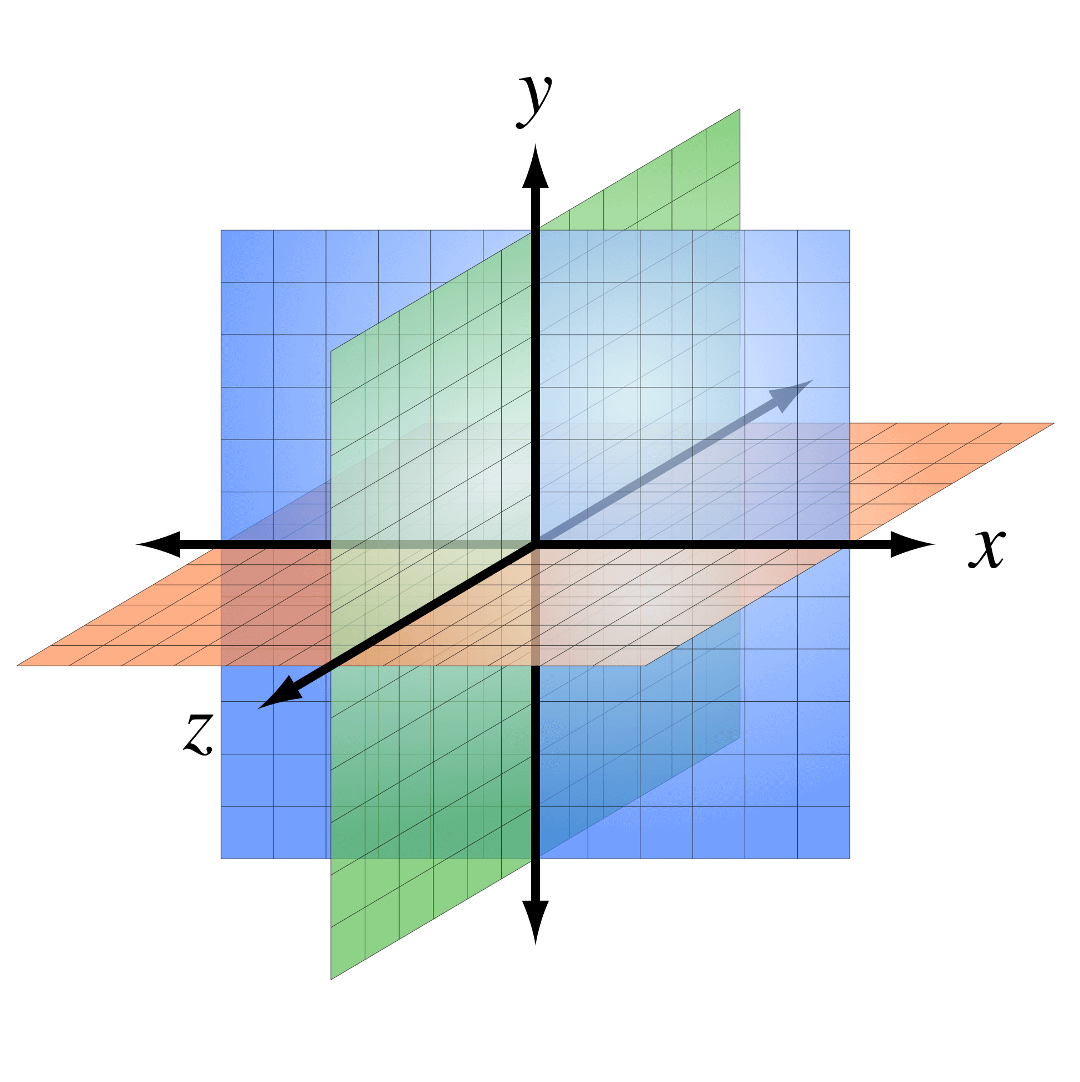
\includegraphics[width=.4\textwidth]{figure/coordinate.png}
    \caption{操纵空间坐标系}
    \label{fig-3-3}
\end{figure}

为了减小操作负担和学习难度,我们都尽可能采用眼动进行主导的操纵,并且尽量不引入更多的操纵模态。为了便于接下来对具体操纵方法的阐释,我们在对象操纵空间中设置了一个三维直角坐标系,见图\ref{fig-3-3}。

\subsection{空间位移}

在空间位移时,对于X-Y平面的移动,对象跟随眼动向前射线在X-Y平面的投影距离作出相应的动作;假设眼动向前射线在X-Y平面的投影坐标为 $(x, y)$ ,对象在X轴向和Y轴向的移动为:

\begin{equation}
	\label{formula-3-2}
	\delta_x = 
    \left\{
    \begin{array}{l}
        0, \quad {\mbox{\boldmath $if$}}\ \left|x\right| < T \\ [0.2cm]
        x \cdot C,\quad {\mbox{\boldmath $default$}}
    \end{array}
    \right.
\end{equation}

\begin{equation}
	\label{formula-3-3}
	\delta_y = 
    \left\{
    \begin{array}{l}
        0, \quad {\mbox{\boldmath $if$}}\ \left|y\right| < T \\ [0.2cm]
        y \cdot C,\quad {\mbox{\boldmath $default$}}
    \end{array}
    \right.
\end{equation}

其中 $T$ 和 $C$ 分别是预先规定的阈值和比例系数。对于Z轴方向的移动,对象跟随头部以Z轴为旋转轴的角度-距离映射作出相应的动作;假设头动绕Z轴的旋转角度为 $\omega$ ,对象在Z轴方向的移动为:

\begin{equation}
	\label{formula-3-4}
	\delta_z = 
    \left\{
    \begin{array}{l}
        0, \quad {\mbox{\boldmath $if$}}\ \left|\omega\right| < T \\ [0.2cm]
        \sin{\omega} \cdot C,\quad {\mbox{\boldmath $default$}}
    \end{array}
    \right.
\end{equation}

其中 $T$ 和 $C$ 分别是预先规定的阈值和比例系数。

\subsection{空间定轴旋转}

在空间旋转时,对于以X轴的旋转,对象跟随眼动向前射线在Y轴的投影距离-角度映射作出相应的动作;对于以Y轴的旋转,对象跟随眼动向前射线在X轴的投影距离-角度映射作出相应的动作;假设眼动向前射线在X-Y平面的投影坐标为 $(x, y)$ ,对象在绕X轴向和Y轴向的旋转为:

\begin{equation}
	\label{formula-3-5}
	\delta_y = 
    \left\{
    \begin{array}{l}
        0, \quad {\mbox{\boldmath $if$}}\ \left|y\right| < T \\ [0.2cm]
        \frac{180}{\pi} \cdot x \cdot C,\quad {\mbox{\boldmath $default$}}
    \end{array}
    \right.
\end{equation}
 
\begin{equation}
	\label{formula-3-6}
	\delta_y = 
    \left\{
    \begin{array}{l}
        0, \quad {\mbox{\boldmath $if$}}\ \left|y\right| < T \\ [0.2cm]
        \frac{180}{\pi} \cdot y \cdot C,\quad {\mbox{\boldmath $default$}}
    \end{array}
    \right.
\end{equation}

其中 $T$ 和 $C$ 分别是预先规定的阈值和比例系数。

\subsection{空间等比例缩放}

在空间缩放时,对象跟随眼动向前射线在X轴的投影距离-缩放系数映射作出相应的动作;假设眼动向前射线在X轴的投影坐标为 $(x, 0)$ ,对象的缩放系数 $K$ 被计算为:

\begin{equation}
	\label{formula-3-7}
	K = 
    \left\{
    \begin{array}{l}
        0, \quad {\mbox{\boldmath $if$}}\ \left|y\right| < T\ {\mbox{\boldmath $or$}}\ x \le -1 \\ [0.3cm]
        2, \quad {\mbox{\boldmath $if$}}\ \frac{x}{C} \ge 1 \\ [0.2cm]
        1 + \frac{x}{C},\quad {\mbox{\boldmath $default$}}
    \end{array}
    \right.
\end{equation}

其中 $T$ 和 $C$ 分别是预先规定的阈值和比例系数。基于此缩放系数,对象放缩的最终具体表现为 $Scale^\prime = Scale \cdot K$ 。

\section{信号处理}

\subsection{眼动信号滤波算法}

\begin{algorithm}[t!]
    \caption{针对该交互系统的眼动信号滤波算法}
	\begin{algorithmic}[1]
        \State SAMPLE $\leftarrow$ 5
 
        \State dataBuffer $\leftarrow$ EMPTY LIST of NUMBER
        \State currentBufferSize $\leftarrow$ dataBuffer.Count()

        \If {currentBufferSize $<$ SAMPLE}
        \For {i \textbf{in} Range(SAMPLE - currentBufferSize)}
            \State dataBuffer.Enqueue(GetData())
            \State Delay()
        \EndFor
        \Else
        \State dataBuffer.Dequeue()
        \State dataBuffer.Enqueue(GetData())
        \State Delay()
        \EndIf
        \State
        \State max $\leftarrow$ $-INF$
        \State min $\leftarrow$ $INF$
        
        \For {value \textbf{in} dataBuffer}
            \State max $\leftarrow$ value \textbf{if} value $>$ max \textbf{else} max
            \State min $\leftarrow$ value \textbf{if} value $<$ min \textbf{else} min
        \EndFor

        \State dataBuffer.RemoveFirst(max)
        \State dataBuffer.RemoveFirst(min)  

        \
        \State sum $\leftarrow$ 0
        \For {value \textbf{in} dataBuffer}
            \State sum $\leftarrow$ sum + value
        \EndFor
        \State \Return sum $/$ (SAMPLE -2 )
	\end{algorithmic} 
	\label{algorithm-3-1}
\end{algorithm} 

基于眼动的对象操纵方法的一大难点即眼动信号不稳定。其原因为:(1)眼部肌肉本能动作(如眨眼、跳视等)干扰频繁,引入大幅度的离群噪声信号,导致眼动信号解析难度大;(2)目前的眼动追踪设备信号无法做到采样率和分辨率的平衡,导致设备无法兼顾运算速度和捕捉精度,并且时常会出现随机的脉冲干扰。所以,我们为此提出了一种针对该交互系统的眼动信号滤波算法,让追踪设备可以在最低硬件消耗的基础上做到低噪声、平滑的眼动信号捕捉,见算法\ref{algorithm-3-1}。

该滤波算法基于中位值平均滤波法。中位值平均滤波算法是一种常用的数字信号处理方法,它结合了中位值滤波和算术平均滤波的优点,能有效地抑制脉冲噪声和周期性干扰,提高信号的平滑度和稳定性。中位值平均滤波算法的基本思想是:对于给定的一组采样数据,先去掉其中的最大值和最小值,然后对剩余的数据求算术平均值,作为该组数据的滤波输出。中位值平均滤波算法的优点有以下几个方面:(1)它能有效地消除由偶然出现的脉冲性干扰所引起的采样值偏差,保证了信号的真实性;(2)它对周期性干扰有良好的抑制作用,能够保留信号的基本特征;(3)它具有较高的平滑度,适用于高频振荡的系统;(4)该算法不需要排序,计算成本较低且反馈速度较快。

对于交互系统的某一时刻 $n$,我们对其前 $SAMPLE$ 帧接收的眼动信号采用中位值平均滤波算法,并将其返回值作为第 $n + 1$ 帧接收的眼动信号。

\subsection{平滑交互处理}

在目标选择以及操纵时,单纯依靠眼动或者头动的某一单一信号是不理想的;完全独立眼动和头动信号会使得交互流程不够自然,且很难实现微小幅度的交互动作,无法避免地会引入不必要的使用负担。因此,我们引入了一种头眼协同的信号处理函数,为交互过程引入更小的负担,使交互流程更加平滑。

平滑交互处理的核心思想即优化对凝视驻留点的计算方式。我们规定在 $t_0$ 时刻的眼动操纵注视停留 $OE$ 被计算为在时间段 $n$ 内的眼动向前射线和头动向前射线的配合角度偏移:

\begin{equation}
	\label{formula-3-8}
	OE_{t_0} = \frac{1}{n} \sum_{t=t_0-n}^{t_0} \left| \hat{eye_t} \cdot \hat{head_t} - \hat{eye_{t-1}} \cdot \hat{head_{t-1}} \right|
\end{equation}

其中,$\hat{eye}$ 是视线的单位向量,$\hat{head}$ 是头部注视的单位向量,$\cdot$ 是向量内积运算符。如果 $OE$ 小于某一阈值,则表示用户正在尝试注视。我们的一个先导实验表明,这个优化是必要的;它可以让交互流程更加平滑自然,引入更小的使用负担。
% !Mode:: "TeX:UTF-8"
\chapter{实验设计}

\section{先导实验}

\subsection{实验1:眼动确认信号筛选}

\subsection{实验2:眼动操纵视线驻留检测优化}

\section{用户实验}

\subsection{实验1:单物体位移对接实验}

\subsection{实验2:单物体操纵对接实验}


% 致谢
% !Mode:: "TeX:UTF-8"
\chapter*{致谢}
\addcontentsline{toc}{chapter}{致谢}

来到北航之后,从士谔书院到计算机学院,我写过无数的代码。这么些年,代码改变了世界,也改变了我。在本科的尾声中,我也想以这个形式书写我的致谢:

%New colors defined below
\definecolor{codegreen}{rgb}{0,0.6,0}
\definecolor{codegray}{rgb}{0.5,0.5,0.5}
\definecolor{codepurple}{rgb}{0.58,0,0.82}
\definecolor{backcolour}{rgb}{0.95,0.95,0.92}

%Code listing style named "mystyle"
\lstdefinestyle{mystyle}{
  commentstyle=\color{codegreen},
  keywordstyle=\color{magenta},
  numberstyle=\tiny\color{codegray},
  stringstyle=\color{codepurple},
  basicstyle=\ttfamily\footnotesize,
  breakatwhitespace=false,         
  breaklines=true,                 
  captionpos=b,                    
  keepspaces=true,                 
  numbers=left,                    
  numbersep=5pt,                  
  showspaces=false,                
  showstringspaces=false,
  showtabs=false,                  
  tabsize=2
}

%"mystyle" code listing set
\lstset{style=mystyle}
\begin{lstlisting}[language=Python, frame=none]
from time import sleep


def thanks_parents():
    print('致父母:')
    print('感谢我的父母在本科四年一直以来的精神支持,'
          '义无反顾地信任我的每个判断和决定,让我随时充满自信;'
          '感谢我的父母在本科四年一直以来的经济支持,让我可以衣食无忧地专注于学业。'
          '我永远不会忘记你们的每一通电话的问候和每一箱寄来的水果。\n')


def thanks_soulmate():
    print('致文珩:')
    print('感谢我的伴侣在我的本科期间对我始终如一的勉励和信任,'
          '也感谢我们在2019年立下的约定。'
          '如果没有这个约定,我可能不会在每次计组实验那么卖力,'
          '可能不会在朋友们都去嗨皮的时候去联系科研机会。'
          '是这个约定支撑我翻过每一个看似不可逾越的大山,'
          '是你不变的陪伴激励我爆发出自己最大的可能性。'
          '虽然本科四年有一半以上的时间我们之间都隔着半个地球的距离,'
          '但是若心联结,殊途终会同归。'
          '回望四年,每一次分别和重逢,每一次欢喜和悲伤,都万分值得。\n')


def thanks_teachers():
    print('致老师:')

    teachers = ['王莉莉教授', 'Prof. Xing-Dong Yang', '李俊教授', 'Prof. Jian Zhao', '徐枫教授']
    institutions = ['北京航空航天大学', 
                    'Simon Fraser University', 
                    '北京师范大学', 
                    'University of Waterloo', 
                    '清华大学']

    teacher_dict = {i: t for i, t in zip(institutions, teachers)}

    for i, t in teacher_dict.items():
        print("我想对{0}的{1}致谢。".format(i, t), end='')
        print(
            '感谢王老师在我的漫漫求索中为我提供的莫大帮助和对我的研究能力的培育。'
            '在虚拟现实实验室的日子可以算是我本科最有意义的日子,'
            '因为我在这里确定了自己的兴趣方向。' 
            if t == '王莉莉教授' else
            '感谢Prof. Yang在几乎素不相识的情况下信任并接纳我进入他的人机交互实验室,'
            '并且总是像关切自己的学生一样询问我的近况和难处。'
            '这段经历使我充分坚定了出国深造的决心。' 
            if t == 'Prof. Xing-Dong Yang' else
            '感谢李老师在我的本科期间带领我发表了第一篇国际学术论文,'
            '让我体会到学术研究能够带给我的无限乐趣和成就感。' 
            if t == '李俊教授' else
            '感谢Prof. Zhao对我学术能力的认可,为我提供宝贵的研究生学习机会。'
            if t == 'Prof. Jian Zhao' else
            '感谢徐老师在我大一时慷慨地为我提供有关计算机视觉和图形学的教导;'
            '徐老师潜移默化教授给我的方法与理念影响了我整个本科的学习思路和历程。\n' 
            if t == '徐枫教授' else '')


def thanks_seniors():
    print('致前辈:')

    seniors = ['刘小龙博士', '徐哲尔博士']
    institutions = ['北京航空航天大学', 'Dartmouth College']

    senior_dict = {i: t for i, t in zip(institutions, seniors)}

    for i, t in senior_dict.items():
        print("我想对{0}的{1}致谢。".format(i, t), end='')
        print(
            '感谢小龙师兄在科研中对我的各种问题不厌其烦的解答。' 
            if t == '刘小龙博士' else
            '感谢哲尔师兄在暑期研究中带领我有条不紊地攻破一个个难点。\n' 
            if t == '徐哲尔博士' else '')


def thanks_music():
    print('致音乐:')
    print('感谢北航交响乐团,让我在本科四年时间里一直有机会坚持自己的爱好,'
          '让我可以在紧张忙碌的课业之余享受音乐、卸下负担。\n')


def thanks_opportunities():
    print('致机会:')
    print('感谢所有我遇到的机会,机会即是一切。\n')


def thanks_me():
    print('致自己:')
    print('感谢自己,从未放弃任何大小之事。\n')


if __name__ == '__main__':
    thanks_parents()
    sleep(5)
    thanks_soulmate()
    sleep(5)
    thanks_teachers()
    sleep(5)
    thanks_seniors()
    sleep(5)
    thanks_music()
    sleep(5)
    thanks_opportunities()
    sleep(5)
    thanks_me()
    
\end{lstlisting}
\cleardoublepage

% 参考文献
% !Mode:: "TeX:UTF-8"
\cleardoublepage
\phantomsection
\addcontentsline{toc}{chapter}{参考文献}
\nocite{*}
\bibliography{bibs}
\cleardoublepage

% 附录
% \appendix
% % !Mode:: "TeX:UTF-8"
\chapter{常见问题}
\label{chapter-faq}
\begin{enumerate}
\item 本模板如何使用?
\label{faq-howtouse}
\begin{itemize}
    \item 按照第2章的要求,先下载和安装相应的软件,推荐使用\TeX{}Live2012或更新的版本;
    \item 下载cls文件;
    \item 使用tex的编辑器或其他编辑器,编写论文,注意保存为UTF-8编码;
    \item xelatex编译。
\end{itemize}
注意:\TeX{}Live2012的ISO镜像在\href{http://buaabt.cn/showtopic-214948.aspx}{未来花园BT站}上
有相应的种子可下载,亦可从TUG的\href{http://www.tug.org/texlive/acquire-iso.html}{官方网站}上下载。
\item Windows下的msmake.bat如何使用?
\label{faq-msmake}
\begin{itemize}
    \item 使用Windows的CMD命令行,进入到msmake.bat所在目录;
    \item 键入~msmake~后会显示相应的帮助文件;
    \item 按照所显示的相关信息再键入相应命令即可。
\end{itemize}
注意:由于此批处理文件为编者自行编写,学识有限,代码有许多不如人意之处,
如对此批处理文件有问题可直接邮件联系我(mrpeng000@gmail.com)即可。
\item 使用TexLive如何更新?
\label{faq-texliveupdate}
TUG官方推荐\TeX{}Live通过镜像站进行更新,具体步骤为:
\begin{itemize}
    \item 在“开始”目录下的TeXLive2012文件夹下,找到有TeX Live Manage程序;
    \item 在菜单“tlmgr”下选择“载入其他仓库”,选择最近的仓库即可(如果是北航校内用户并能够
    访问到\href{http://mirror.buaa.edu.cn/}{北航开源镜像站}的话,可以在仓库地址中
    输入\texttt{http://mirror.buaa.edu.cn/CTAN/systems/texlive/tlnet/});
    \item 按照目录选择更新。
\end{itemize}
\end{enumerate}

% % !Mode:: "TeX:UTF-8"
\chapter{联系我们}

\end{document}
